\documentclass{article}
\usepackage{fancyhdr}
\usepackage{array} 
\usepackage[a4paper, left=1in, right=1in, top=1in, bottom=1in]{geometry}
\usepackage{graphicx}  
\usepackage{appendix}
\usepackage{amsmath}
\usepackage{amssymb}
\usepackage[font=small,it]{caption}
\usepackage{float}
\usepackage{xcolor}
\usepackage{tikz}
\usepackage{longtable,tabularx}
\usepackage{booktabs}
\usepackage[table]{xcolor}
\usepackage{subcaption}
\usepackage{pdflscape}
\usepackage{pdfpages}
\usepackage{changepage} % pour adjustwidth si besoin
\captionsetup[longtable]{position=bottom}
\usepackage[backend=biber, style=numeric, sorting=none]{biblatex}
\AtEveryBibitem{\clearfield{note}}
\addbibresource{references.bib}
\usepackage[colorlinks=true, linkcolor=blue, urlcolor=black, citecolor=blue]{hyperref}


\begin{document}

\begin{titlepage}

    \centering
    \begin{figure}[H]
        
\includegraphics[width=0.3\linewidth]{Photos/epfl.png}
    \end{figure}

    \noindent\rule{\textwidth}{0.5pt}

    \begin{center}    
        \Large ‘Products Design and Systems Engineering in a Team’\\[0.2cm]
        Microengineering Section, Master Phase Fall 2025
    \end{center}

    \noindent\rule{\textwidth}{0.5pt}
    \vspace{2.8cm}
      
    {\Huge \textbf{THINK WATER}}

    % -------- LOGO PROJET --------
    \vspace{0.8cm}
    \begin{center}
        
\includegraphics[width=0.6\textwidth]{logos/logo_sans_text.png}
    \end{center}
    % ----------------------------

    \vspace{1cm}

    \begin{center}
        {\large
        \textbf{Group 2 :}\\[0.8em]
        Mostafa Zaki, 356944\\[0.4em]
        Mathieu Dubois, 313367 \\[0.4em]
        Martin Samuel Draï, 316708\\[0.4em]
        Eliot Cloutier, 346992 \\[0.4em]
        Estezet Roméo Clément, 420762}
    \end{center}

    \vspace{1.5cm}
    \noindent\rule{\textwidth}{0.5pt}

    {\large
    \textit{Professors :} \hfill Edoardo Charbon, Yves Bellouard\\[0.5em]
    \textit{Teaching assistant :} \hfill Nicolas Robson}

    \noindent\rule{\textwidth}{0.5pt}

\end{titlepage}


\newpage
\pagenumbering{gobble}
{\hypersetup{linkcolor=black}
\tableofcontents
}
\newpage
\pagestyle{fancy}
\fancyhf{}
\renewcommand{\headrulewidth}{0.4pt}
\fancyhead[L]{
\includegraphics[height=0.9cm]{Photos/epfl.png}}
\fancyhead[R]{\nouppercase{\rightmark}}
\fancyfoot[C]{\thepage}
\renewcommand{\sectionmark}[1]{\markright{#1}}

\pagenumbering{arabic}
\setcounter{page}{1}
% ============================================================
% Executive summary
% ============================================================
\section*{Executive Summary}
\addcontentsline{toc}{section}{Executive summary}
\markboth{Executive summary}{Executive summary}
Dehydration is a widespread but often underestimated issue among elderly people living independently. Many seniors do not consciously monitor their daily water intake, and dehydration is frequently identified only once it becomes an aggravating factor in hospitalization. The purpose of this project is to design a simple, non-invasive, and domestic hydration monitoring solution adapted to seniors, while preserving their daily habits. The proposed product targets the growing senior population living at home, a market segment that is expanding rapidly and remains largely underserved by existing solutions.\vspace{0.2cm}

The result of this work is the "Think Water" device, a personal hydration monitoring system composed of two physical devices: a smart coaster and a base station. The coaster is placed under any glass and measures water intake automatically during daily use. It detects drinking events through weight variation and motion analysis, then communicates the information wirelessly to the base station. The base station retrieves data, computes personalized daily hydration targets, stores long-term history, and provides feedback to the user through screen and audio stimuli. This architecture allows accurate hydration tracking without requiring any smartphone, application, or active user interaction.\vspace{0.2cm}

From a technical perspective, the project focused on several key challenges. Accurate sip detection was achieved using a multi-sensor approach combining a load cell, an inertial measurement unit, and a glass presence detection (with a hall sensor), ensuring reliability in real domestic conditions with any type of glass. A low-power architecture was implemented by splitting the system into two devices: a battery powered coaster optimized for autonomy and a base station responsible for computation, display, and feedback. Bluetooth Low Energy communication (BLE), local data storage, and a simple user interface were chosen to maximize usability and robustness, particularly for elderly users.\vspace{0.2cm}

In terms of market positioning, the "Think Water" differentiates itself clearly from existing solutions. Unlike smart bottles or app-based hydration trackers, it does not impose a specific container, does not rely on digital literacy, and does not require habit changes. The key unique selling point of the product is its adaptability both in terms of hydration target customization and in the use of different glass types. The objective is computed for each user based on personal and environmental parameters rather than generic recommendations. This positioning, combined with a discreet and domestic-oriented design, creates a strong value proposition with limited direct competition.\vspace{0.2cm}

From an intellectual property perspective, a detailed prior art and patent analysis highlighted both existing solutions and clear opportunities for differentiation. While several patents address hydration reminders or consumption tracking, none combine a detachable measurement unit attached to the glass with a fully local, two-device architecture and personalized hydration targets. Our approach avoids reliance on cloud services or mobile applications and introduces a novel separation of functions between a smart coaster and a physical base station. In addition, the personalization model used to compute hydration goals represents a strong differentiating element that can be protected as a trade secret, while the overall system architecture and attachment mechanism offer opportunities for patent protection. This analysis confirms both freedom to operate and a solid basis for a defensible IP strategy.\vspace{0.2cm}



The prototype made demonstrates the core elements of the product concept: automatic sip detection, personalized hydration goals, local data storage, intuitive feedback, and senior-friendly interaction. While not yet a final product, it validates the technical feasibility and relevance of the concept. The project was carried out through a structured team effort, with clear task allocation between mechanical design, electronics, software development, and project management. Iterative prototyping, testing, and coordination allowed the team to overcome manufacturing delays and integration challenges.\vspace{0.2cm}

Looking forward, several improvements have been identified to move toward a market-ready product. These include further miniaturization, a simplified attachment mechanism, splash-proof or waterproof design, wireless charging, enhanced display functionalities, and optional secure remote data access for caregivers or healthcare professionals. Obtaining medical-grade certification is also considered a long-term objective to increase credibility and market impact.\vspace{0.2cm}

In conclusion, this project successfully delivered a functional prototype that addresses a real and growing societal need. "Think Water" offers a novel, practical, and scalable approach to domestic hydration monitoring. With further development and refinement, it has strong potential to evolve into a viable commercial product and a meaningful contribution to preventive healthcare for seniors.

\newpage

% ============================================================
% I. PRODUCT CONCEPT
% ============================================================
\section{Product Concept}

\subsection{General Description}

"Think Water" is composed of two main elements: the coaster and the base station.
\vspace{0.5cm}



\begin{figure}[H]
    \centering
    \begin{minipage}{0.3\textwidth}
        \centering
        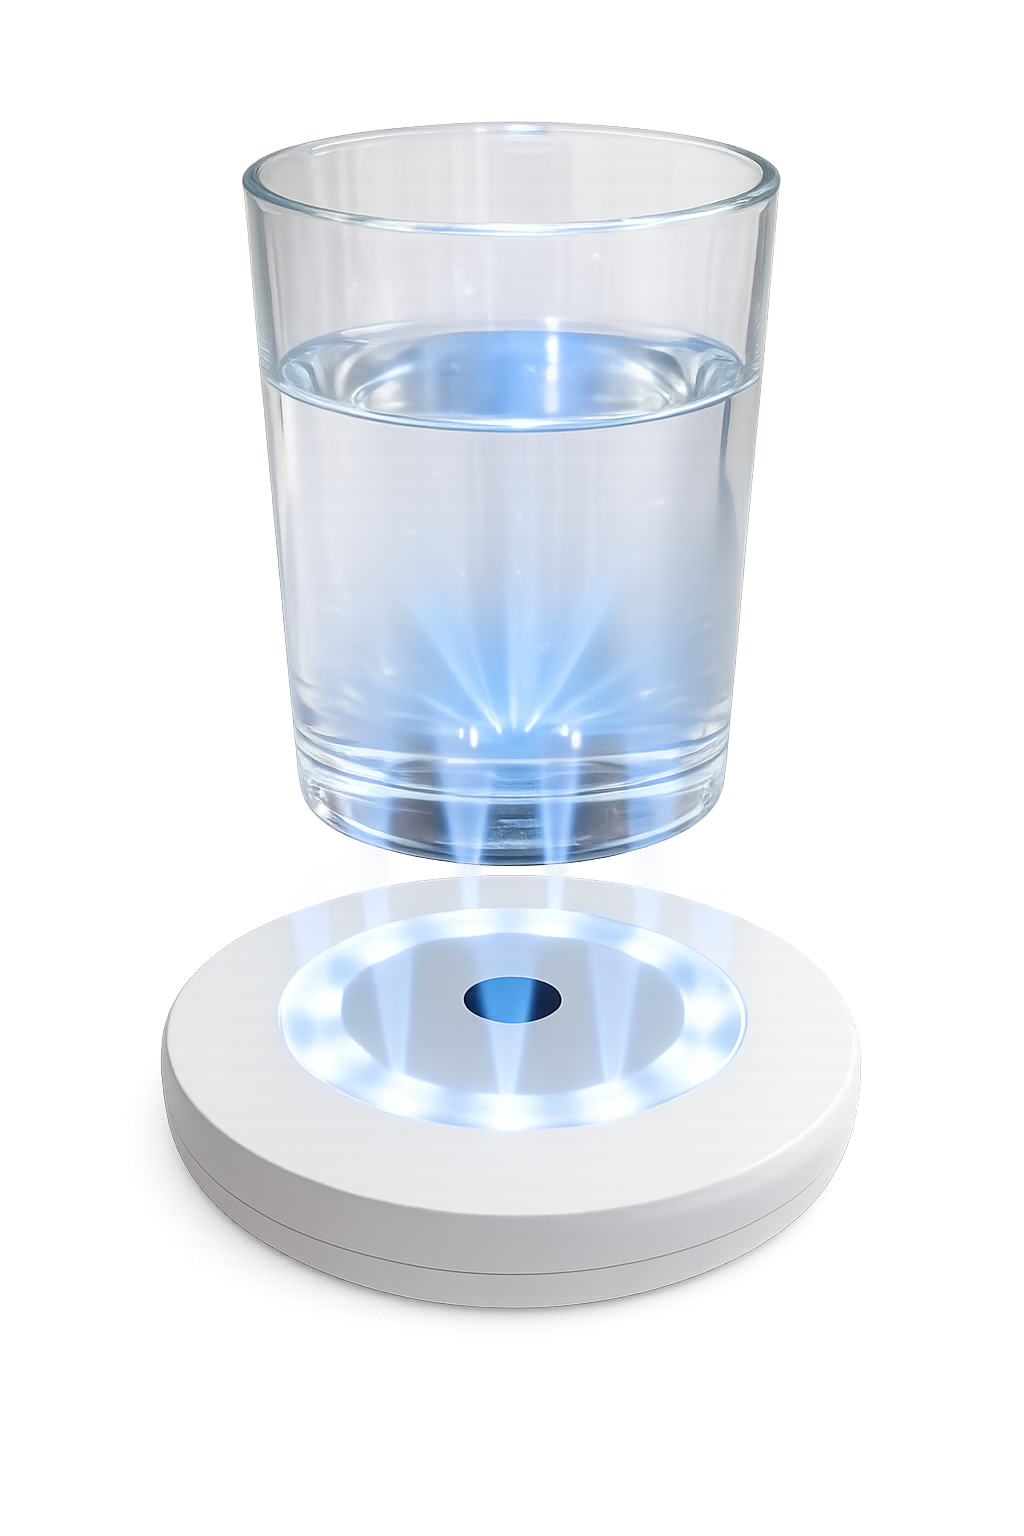
\includegraphics[height=6cm]{Photos/coaster_remove.png}
        \caption{The coaster}
        \label{fig:coaster}
    \end{minipage}
    \hfill
    \begin{minipage}{0.6\textwidth}
        \centering
        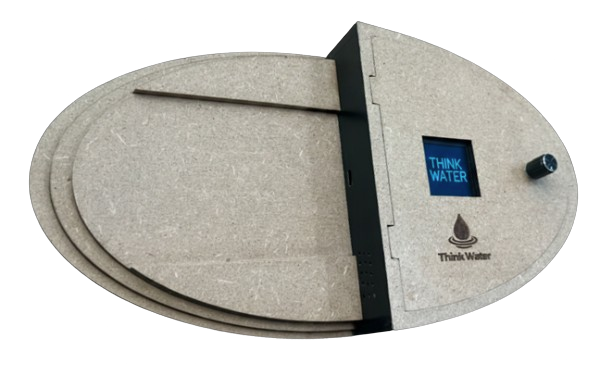
\includegraphics[height=6cm]{Photos/base_station-remove.png}
        \caption{The base station}
        \label{fig:base_station}
    \end{minipage}
\end{figure}


The coaster is a compact, circular, and detachable device designed to fit beneath the user’s glass. The base is a small home unit that collects environmental data, communicates with the coaster, and also serves as a charging station.\vspace{0.2cm}  

During setup, the user enters basic personal information such as age, sex, and weight directly on the base using the screen and control knob. These information along environmental data allows the system to calculate an individual daily hydration target.  
\vspace{0.2cm} 

The coaster measures water consumption in less than one second using a precise pressure sensor. It communicates wirelessly with the base station within a range of about 20 meters. Visual feedback is provided through LEDs that light up when the glass is lifted, showing the user progression on its hydration target (blue lights), or when the user’s water intake is below the recommended level (red light), while the base provides an audio reminder through a buzzer. All data is stored locally on the base, which can record up to 2 GB of information to monitor hydration trends and weekly averages. The coaster operates independently for more than a week before needing to be recharged, and it can be placed on the base station to charge when necessary.\vspace{0.2cm} 

On the base’s LCD screen, the user can see their progress, including total water intake, daily averages, and personalized goals. Sensors on the base measure temperature and humidity to adjust the hydration target depending on environmental conditions.\vspace{0.2cm}  

From the user’s point of view, the product package includes the coaster, the base, power cables, and few small magnetic plates with adhesive VHB tape to attach under glasses, allowing for a stable yet discreet connection. Once set up, the experience is straightforward: the user places his glass on the coaster and drinks normally. The coaster automatically measures the volume of water consumed, will remaining attached to the glass using the magnets, and sends the data to the base in real time.\vspace{0.2cm} 

This system is designed to fit naturally into the user’s routine, providing gentle reminders and accurate monitoring to encourage regular hydration without disrupting daily life.
\newpage
\subsection{Brief Market Analysis}
In Switzerland, dehydration is a significant public health issue. According to doctors we were able to \hyperref[appendix:interview]{interview}, dehydration is not often the principal cause of hospitalization, but very often, it is an aggravating factor. Studies show that 20\% of people over 75 years old drink less than 1 liter per day \cite{Senso5}, and the situation is even more concerning in retirement homes, where over 50\% of residents consume less than the minimum recommended 1.5 L/day, highlighting a clear market need \cite{EMS}.\\
Thus we can see that elderly people are subject to a problem that can be life threatening. This is why we decided to try build a product to help them remember to drink in order to try to prevent extreme cases.

\subsection{Unique Selling Points of the Product}

The following diagram summarizes the Unique Selling Points (USP) of our product,
highlighting what differentiates it from competitors and why it fits the users' needs.

\begin{figure}[H]
    \centering
    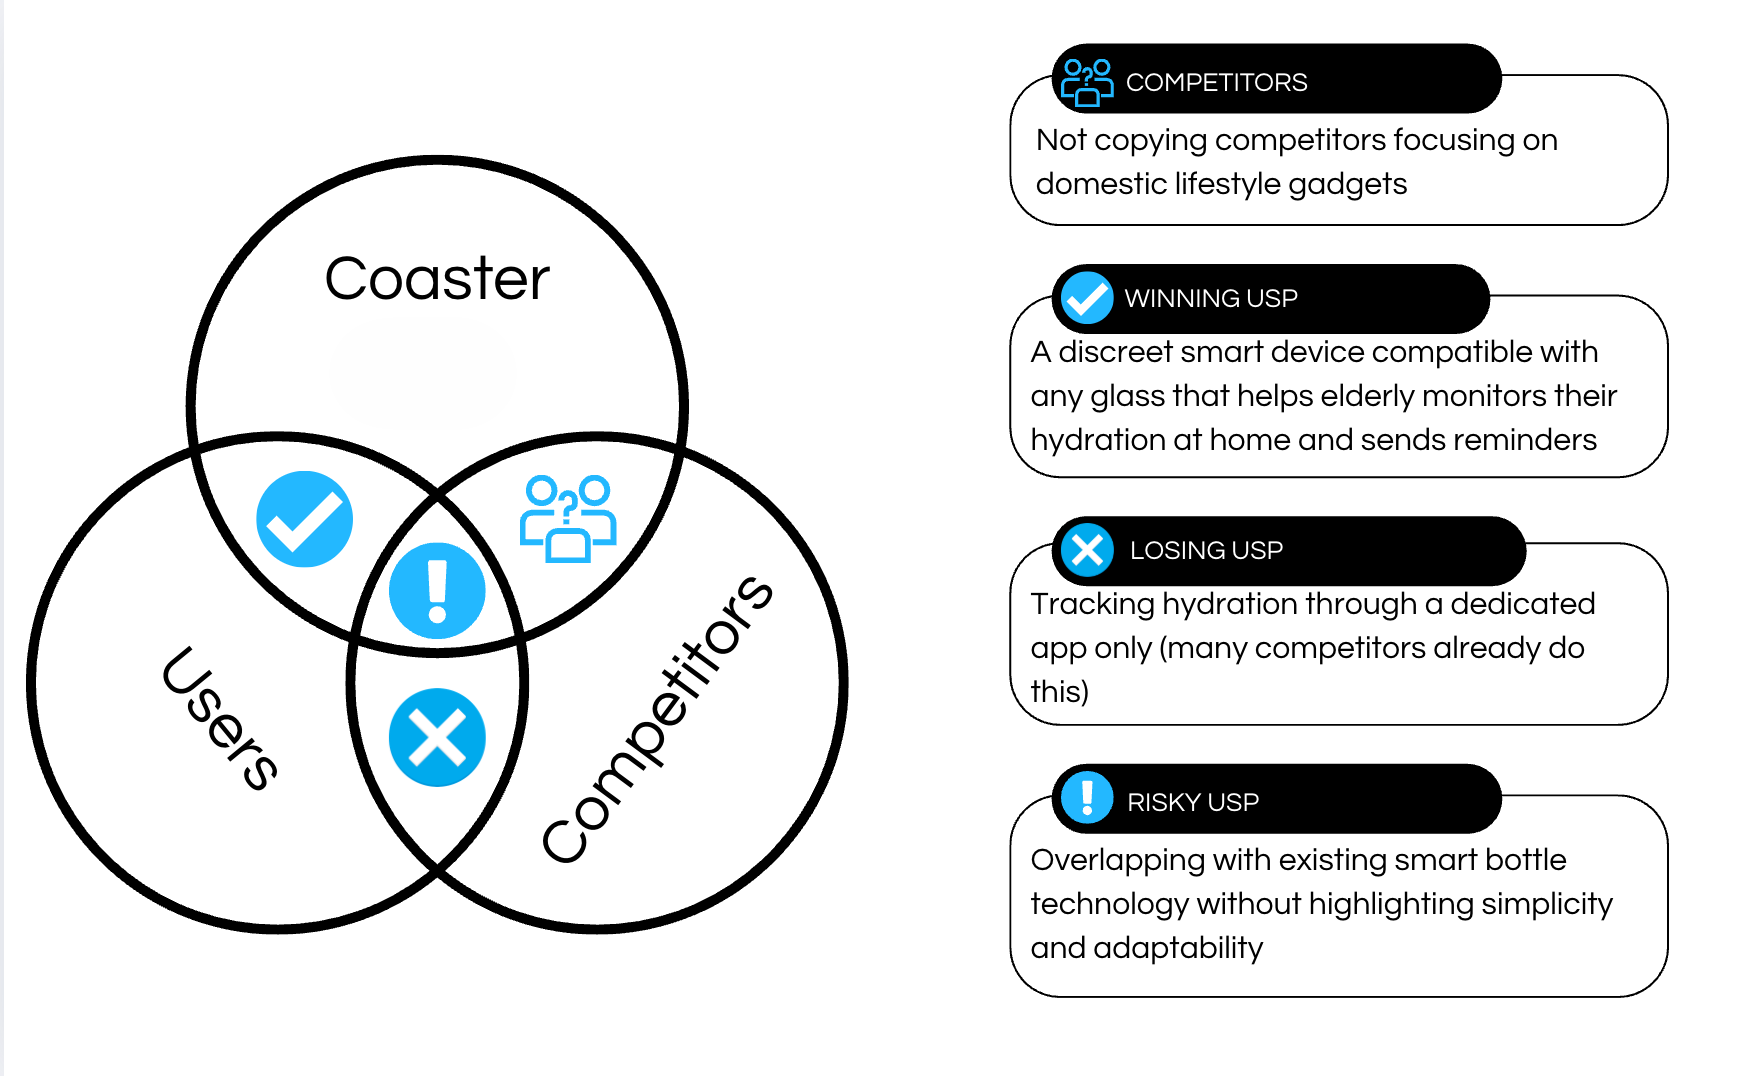
\includegraphics[trim = 0.2cm 0cm 0cm 0cm,
  clip, width=0.85\textwidth]{logos/usp.png}
    \caption{Unique Selling Points (USP) analysis of the "Think Water"}
\end{figure}
A lot of companies are doing hydration sensors and device that reminds people to drink. Mostly based on software and digital application, or all-in-one devices. Nevertheless, no companies is making product specifically for domestic use, meaning discrete, ergonomic and easy-to-use. Moreover, no companies have personalized targets for individuals, which is also a key feature of our product. 
To be personalized it requires some easy pre-steps before starting but once it is done, it ensures freedom of use to the customer. The fact that our device is separated in 2 parts, allows us to make a smaller coaster, while keeping record of the water consumption and displaying it dynamically to the customer on the base station. Not only it reminds you to drink based on your specific needs, but it also ensures that you can use it easily and, importantly, with any glass you have at home. This strength is something unique that will motivate the customers to buy our product. Having a device that is made for domestic use but not invasive and adaptable will allow the customer to change its habit in a reasonable way. It is the key point of our product. We focused our efforts in making something discrete but yet precise, personalized and adapted to domestic use and to seniors. This novelty is what will attract customers and allow us to enter the market with confidence.
\newpage

% ============================================================
% II. TECHNICAL SOLUTION
% ============================================================
\section{Technical Solution}
\markboth{Technical solution}{Technical solution}

This section summarizes the key functional and technical specifications of our prototype.  
The main engineering requirements are grouped by functionality in Tables~\ref{tab:reqs}.  
Each functionality is assigned a letter code for clarity, as indicated below. For the components code refer to section \ref{subsec:design}.

\vspace{0.3cm}

\noindent\textbf{Legend:}  
\textcolor{cyan!60!black}{\textbf{C}} – Communication \hspace{0.8cm}
\textcolor{orange!90!black}{\textbf{M}} – Measurement \hspace{0.8cm}
\textcolor{green!60!black}{\textbf{P}} – Power \hspace{0.8cm}
\textcolor{violet!70!black}{\textbf{U}} – User Interface \hspace{0.8cm}
\textcolor{gray!70!black}{\textbf{S}} – Structure


\renewcommand{\arraystretch}{1.2}
\setlength{\tabcolsep}{3pt}
\setlength\LTleft{0pt}
\setlength\LTright{0pt}
\rowcolors{3}{blue!5}{white}

\begin{longtable}{
  |>{\centering\arraybackslash}m{0.9cm}
  |>{\centering\arraybackslash}m{2.8cm}
  |>{\centering\arraybackslash}m{1.6cm}
  |>{\centering\arraybackslash}m{2.3cm}
  |>{\centering\arraybackslash}m{1.7cm}
  |>{\centering\arraybackslash}m{1.3cm}
  |>{\centering\arraybackslash}m{1.4cm}
  |>{\centering\arraybackslash}m{1.4cm}
  |>{\centering\arraybackslash}m{1.2cm}|
}
\caption{\textbf{Engineering Requirements Table}}\label{tab:reqs} \\
\hline
\rowcolor{blue!25}
\textbf{Func.} & \textbf{Function} & \textbf{Comp \#} & \textbf{Metric} & \textbf{Unit} & \textbf{Priority} & \textbf{Min} & \textbf{Max} & \textbf{Result} \\
\hline
\endfirsthead

\hline
\rowcolor{blue!25}
\textbf{Func.} & \textbf{Function} & \textbf{Req \#} & \textbf{Metric} & \textbf{Unit} & \textbf{Priority} & \textbf{Min} & \textbf{Max} & \textbf{Result} \\
\hline
\endhead

\hline
\multicolumn{9}{|r|}{\small Continued on next page} \\
\hline
\endfoot

\hline
\endlastfoot

% ===== COMMUNICATION =====
\rowcolor{cyan!10}
C1 & Communication between coaster and base & \#4 & Wireless communication range & m & Shall & 10 & -- & $>$ 20\\ \hline

\rowcolor{cyan!10}
C2 & Communication with external users & \#5 & Internet connection & -- & Should & -- & -- & $\times$ \\ \hline

% ===== MEASUREMENT =====
\rowcolor{orange!10}
M1 & %aquisition time of weight mesurement
Measure water consumption (time) & \#1, \#0, \#3 & Response time & s & Shall & 0 & 1 & 1 \\ \hline

\rowcolor{orange!10}
M2 & Measure weight accurately & \#1,\#3 & Weight measurement error & g & Shall & -- & $\pm$10 & $\pm$1 \\ \hline

\rowcolor{orange!10}
M3 & Measure temperature/humidity & \#13 & Temp/Humidity accuracy & °C / \%RH & Shall & 0°C / 0\% & $\pm$1°C / $\pm$10\% & $\pm$0.1°C / $\pm$1\% \\ \hline

\rowcolor{orange!10}
M4 & Detect glass presence/removal & \#14 & Detection Accuracy & \% & Shall & 95 & -- & Pass \\ \hline

\rowcolor{orange!10}
M5 & Sleep/awake mode control & \#1, \#15 & Stability detection & -- & Should & -- & -- & \checkmark \\ \hline

\rowcolor{orange!10}
M6 & Store all measurements & \#0, \#2, \#16 & Time of storage & h & Shall & 24 & 48 & 48 \\ \hline

\rowcolor{orange!10}
M7 & Compute a daily theoretical consumption target& \#2 & Working target computation & -- & Shall & -- & -- & \checkmark \\ \hline

\rowcolor{orange!10}
M8 & Store daily consumption data and theoretical daily target& \#2, \#16 & Time of storage & Years & Shall & 1 & 2 & 2 \\ \hline

% ===== POWER =====
\rowcolor{green!10}
P1 & Provide power autonomy & \#11 & Battery autonomy &  days & Shall & 7 & 10 & 9 \\ \hline

\rowcolor{green!10}
P2 & Charge the coaster & \#12 & Easy to charge & -- & Shall & -- & -- & \checkmark \\ \hline

\rowcolor{green!10}
P3 & Provide power to the base & \#12 & Input voltage stability & -- & Shall & -- & -- & \checkmark \\ \hline

% ===== USER INTERFACE =====
\rowcolor{violet!10}
U1 & Visual reminder & \#6 & Light intensity & Lux (at 30cm) & Shall & 30 & 50 & Pass \\ \hline

\rowcolor{violet!10}
U2 & Audio reminder & \#7 & Sound intensity & dB (at 30cm) & Shall & 65 & 75 & 65 \\ \hline

\rowcolor{violet!10}
U3 & Daily hydration display & \#8 & Display resolution & pixels & Shall & 176×176 & 176×176 & 176×176 \\ \hline

\rowcolor{violet!10}
U4 & Display history & \#2, \#8 & Historic range & days & Should & 7 & 30 & $\times$ \\ \hline



\rowcolor{violet!10}
U5 & User data entry & \#10 & UI implementation & qualitative & Shall & -- & -- & \checkmark \\ \hline

% ===== STRUCTURE =====
\rowcolor{gray!10}
S1 & Coaster-glass magnetic attachment strength & \#17, \#18 & Holding force & N & Shall & 10 & 50 & 10 \\ \hline

\rowcolor{gray!10}
S2 & Shock resistance & \#19 & Drop height resistance & m & Should & 0.5 & 1.5 & casing alone \checkmark \\ \hline

\rowcolor{gray!10}
S3 & Ergonomic circular shape & \#19, \#17 & Diameter & mm & Should & 80 & 120 & 104 \\ \hline

\end{longtable}



\subsection{Design phase: solutions explored}
\subsubsection*{Alternative Solution 1 : Smart Bottle }

\textbf{Description}\vspace{0.2cm}

A first design idea was to develop an all-in-one smart bottle, integrating weight sensing, electronics, battery, and feedback directly inside the bottle. The bottle would automatically measure water intake and remind the user to drink through LEDs or notifications.\vspace{0.2cm}

\textbf{Advantages}
\begin{itemize}
    \item Simple system architecture: all components are embedded in a single object.
    \item Direct measurement of water intake without external calibration.
    \item Common market reference: similar products already exist, making feasibility relatively high.
\end{itemize}

\textbf{Reasons for rejection}\vspace{0.2cm}

Despite its simplicity, this solution was not suitable for domestic and senior use:
\begin{itemize}
    \item It forces users to change their habits by using a specific bottle.
    \item Seniors often have preferred glasses or cups adapted to their needs.
    \item Cleaning, refilling, and portability add constraints.
    \item The product is intrusive in daily life and less discreet.
    \item Already exists.
\end{itemize}

Because our main objective was to create a non-invasive, habit-preserving solution, this option was discarded.

\vspace{0.5cm}

\subsubsection*{Alternative Solution 2 : Fully Software-Based Monitoring (Mobile App Only)}

\textbf{Description}\vspace{0.2cm}

Another approach considered was a software-only solution, where users would manually log their water intake through a mobile application, possibly supported by reminders or notifications.\vspace{0.2cm}

\textbf{Advantages}
\begin{itemize}
    \item No hardware cost, easy to deploy and update.
    \item Scalable solution with cloud-based data access.
    \item Allows advanced analytics and remote monitoring.
\end{itemize}

\textbf{Reasons for rejection}\vspace{0.2cm}

This solution was quickly identified as unsuitable for the target population:
\begin{itemize}
    \item Requires active user engagement, which is unreliable for seniors.
    \item Depends on smartphone ownership and digital literacy.
    \item Manual input leads to low compliance and inaccurate data.
    \item High cognitive load contradicts our goal of an effortless experience.
\end{itemize}

Since our product aims to work in the background without user action, this approach was rejected.



\subsection{Technical Choices Made}

\subsubsection{Selected Design}
\label{subsec:design}

After evaluating multiple design concepts, we selected a dual-device architecture composed of two complementary elements:
\begin{itemize}
    \item a smart coaster that works with any type of glass,
    \item and a base station responsible for computation, display, feedback, and charging.
\end{itemize}

This architecture was chosen as it best addresses the constraints identified during the design phase while preserving a strong level of innovation and technical feasibility.

\subsubsection*{Selection Criteria}

The final concept was selected based on the following criteria:
\begin{itemize}
    \item \textbf{Non-invasiveness}: the solution does not require any change in the user’s drinking habits.
    \item \textbf{Adaptability}: the coaster can be used with any glass available at home.
    \item \textbf{Senior-friendliness}: no smartphone application, no complex interaction, and minimal cognitive load.
    \item \textbf{Technical feasibility}: all components and functionalities could be realistically implemented within the project constraints.
    \item \textbf{Discretion and aesthetics}: the product blends naturally into a domestic environment without drawing attention.
\end{itemize}

This solution offered the best compromise between usability, robustness, and innovation, while remaining realistic to prototype and demonstrate.

\subsubsection*{Functional Architecture}

The selected solution is composed of two physical devices working together:

\begin{enumerate}
    \item \textbf{The base station} receives data from the coaster, computes hydration indicators, stores consumption history, displays information to the user, provides audio and visual feedback through screen, and can hold the coaster to charge it.
    \item \textbf{The coaster} measures the glass weight, detects drinking events, communicates wirelessly with the base using Bluetooth Low Energy (BLE) and give visual feedback through LEDs. 
\end{enumerate}

The list of main hardware components is given in Table~\ref{tab:components}.

\begin{table}[H]
\centering
\renewcommand{\arraystretch}{1.2}
\setlength{\tabcolsep}{12pt}
\begin{tabular}{|c|p{9cm}|}
\hline
\rowcolor{blue!25}
\textbf{Component \#} & \textbf{Name of Component} \\
\hline
\#0  & Microcontroller XIAO nRF52840 Sense\\ \hline
\#1  & Load cell sensor \\ \hline
\#2  & Microcontroller (ESP32 / Adafruit HUZZAH32) \\ \hline
\#3  & Signal amplifier (HX711) \\ \hline
\#4  & BLE communication module (integrated in ESP32 / XIAO) \\ \hline
\#5  & Wi-Fi module (integrated in ESP32) \\ \hline
\#6  & LED indicator \\ \hline
\#7  & Buzzer \\ \hline
\#8  & OLED screen (176×176 px) \\ \hline
\#10 & Rotary knob / encoder \\ \hline
\#11 & Rechargeable Li-ion battery ($\geq$ 820 mAh) \\ \hline
\#12 & Base power supply (USB, 5V and 3.3V) \\ \hline
\#13 & Temperature/Humidity sensor (SHT41) \\ \hline
\#14 & Hall effect sensor \\ \hline
\#15 & Accelerometer (IMU integrated in XIAO) \\ \hline
\#16 & Micro-SD card + SD card reader \\ \hline
\#17 & Magnetic discs (dishwasher-safe) \\ \hline
\#18 & 3M VHB adhesive pads \\ \hline
\#19 & Coaster casing (3D printed) \\ \hline
\#20 & Base station casing (3D printed) \\ \hline
\end{tabular}
\caption{Component list with unique numbering for traceability.}
\label{tab:components}
\end{table}

Detailed circuit diagrams showing the electrical connections and component integration for both the coaster and base station are provided in the appendix (see Figures~\ref{fig:coaster-circuit} and \ref{fig:base-circuit}).\vspace{0.2cm}

The table below summarizes how each functional requirement (C, M, P, U, S) will be addressed in the prototype implementation.

\begin{longtable}{|>{\centering\arraybackslash}m{1cm}|>{\arraybackslash}m{14.5cm}|}
%\caption{Implementation strategy for each functional requirement.}\\
\hline
\rowcolor{blue!25}
\textbf{Func. Code} & \textbf{How we implement the solution} \\
\hline
\endfirsthead

\hline
\rowcolor{blue!25}
\textbf{Func. Code} & \textbf{How we implement the solution} \\
\hline
\endhead

\hline
\multicolumn{2}{r}{\small \textit{Continued on next page}} \\
\endfoot

\hline
\endlastfoot

% ===== COMMUNICATION =====
C1 & Communication between coaster and base is handled using the BLE module integrated in the XIAO nRF52840 Sense (\#0). The coaster sends processed consumption events to the base station at each use. \\
\hline

C2 & External communication (if enabled) uses the Wi-Fi module in the ESP32 HUZZAH32 (\#2) inside the base station to push hydration summaries to a local web dashboard. \\
\hline

% ===== MEASUREMENT =====
M1 & Water consumption is measured using the load cell (\#1), amplified through the HX711 (\#3) and processed by the XIAO (\#0) at high sampling rate with software processing. \\
\hline

M2 & Load cell accuracy is ensured by calibration routine stored in the microcontroller memory (\#0), compensating sensor drift over time. \\
\hline

M3 & Temperature and humidity are captured using the SHT41 sensor (\#13), used by the base station (\#2) to adapt hydration goals automatically. \\
\hline

M4 & Glass placement/removal is detected using the Hall effect sensor (\#14), which triggers events when the magnetic field from the coaster’s magnets changes. \\
\hline

M5 & Stability detection uses load cell readings (\#1) to determine if the coaster is stationary, controlling sleep/wake states. The IMU (\#15) detects motion to trigger LED feedback animations when the glass is lifted. \\
\hline

M6 & All measurements are stored locally on the micro-SD card (\#16) with timestamps, enabling at least 24–48 hours of autonomous logging. \\
\hline

M7 & The microcontroller (\#2) computes a theoretical daily water intake target (around 1.5 L) using a simple algorithm based on user inputs (age, sex, weight) and environmental data (temperature, humidity). \\
\hline

M8 & The microcontroller (\#2) stores the daily consumption data and the theoretical daily target on the micro-SD card (\#16), ensuring a long-term history (1–2 years)  \\

\hline

% ===== POWER =====
P1 & Power autonomy is achieved using a 820 mAh Li-ion battery (\#11)  \\
\hline

P2 & The coaster recharges on the base through a regulated USB-C 5V output converted from the 12V input (\#12). The battery charge is then handled by the built-in charge controller of the XIAO board\\
\hline

P3 & 12V DC input from a wall adapter is converted into 5V and 3.3V powering the different peripherals in the base, and the ESP32 is powered by the same USB 5V converter used for charging the coaster  \\
\hline

% ===== USER INTERFACE =====
U1 & Visual reminders are provided by the LED indicator (\#6), controlled by the microcontroller when hydration is insufficient and low battery detection. \\
\hline

U2 & The buzzer (\#7) emits short audible alerts when the daily hydration objective is not met. \\
\hline

U3 & Daily hydration progress is displayed on the high-resolution OLED screen (\#8). \\
\hline

U4 & Hydration history and graphical feedback are displayed by reading logged data from the SD card (\#16) and rendering simple graphs on the OLED screen (\#8) \\
\hline

U5 & The user uses the knob to enter sex, age and weight. \\
\hline
% ===== STRUCTURE =====
S1 & Attachment strength is achieved by combining magnetic discs (\#17) and VHB adhesive tape under the glass(\#18), ensuring a secure fit between coaster and glass. \\
\hline

S2 & The coaster casing (\#19) is 3D-printed in PETG with a reinforced design to survive drops up to 1.5 m. \\
\hline

S3 & Ergonomic comfort is achieved by designing the coaster diameter (\#19) between 80–120 mm and optimizing the weight distribution. \\
\hline

\end{longtable}

% \end{tabular}


% \end{table}

\subsubsection{Concept of Operation}

\begin{figure}[H]
    \hspace{-1.3cm}
    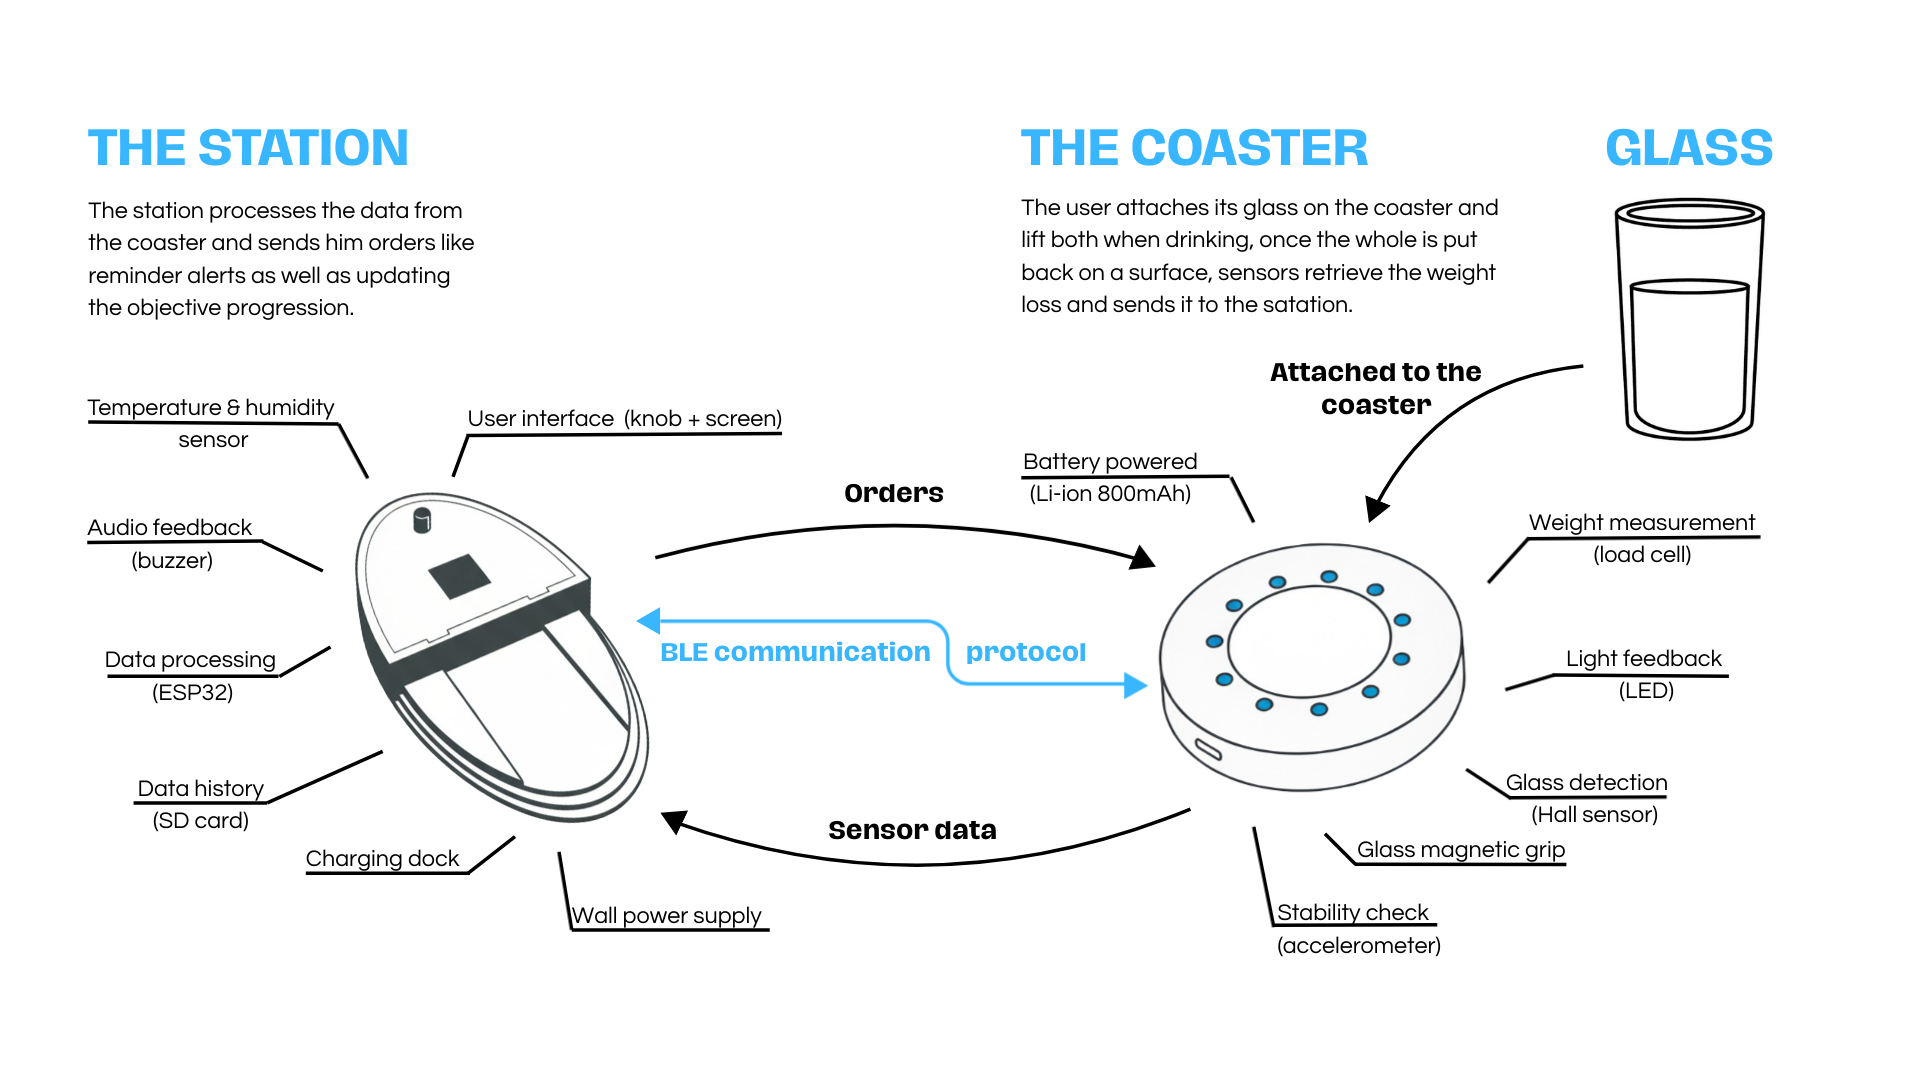
\includegraphics[
        trim=2cm 3cm 2cm 3cm,
        clip,
        width=0.9\paperwidth
    ]{Photos/ConOps.png}
    \caption{Concept of Operation of the product.}
    \label{fig:conops}
\end{figure}

\subsubsection{Key Elements in the Design Related to the USP}

The main USP of our product is the personalization of the daily hydration target. Unlike existing solutions that rely on generic recommendations, our system computes a specific consumption goal for each user using an internal model based on personal and environmental parameters. This makes hydration monitoring more relevant and meaningful. The model was taken from Yamada et al. (2022) \cite{WaterTurnover2022}, a large-scale study published in \textit{Science} involving 5,604 participants from 23 countries, adapted and implemented in our algorithm.\vspace{0.2cm}

Another key design choice is the detachable measurement unit placed directly under the glass. While most existing devices are table-based or integrated into dedicated containers, our coaster allows the user to keep their own glassware. This reduces habit changes and makes the product particularly well suited for domestic and senior use.\vspace{0.2cm}

The feedback system also plays an important role in differentiation. By combining visual feedback on the coaster and audio feedback on the base station, the system ensures that reminders remain effective in various situations, even when the user is not actively interacting with the device.\vspace{0.2cm}

Finally, the use of two physical devices instead of a software or a cloud-dependent solution was a deliberate design choice. It allows advanced functionalities such as data storage, display, adaptability and personalization without requiring a smartphone, improving accessibility and usability for seniors.\vspace{0.2cm}

Potential future optimizations of these design choices are discussed in Section~\ref{sec:perspective}.

\subsubsection{Analysis / Modeling of these Key Elements}

This section presents how the main technical functions of the "Think Water" were modeled, dimensioned, and validated, as well as how these choices could be further optimized in a future version of the product.\vspace{0.2cm}

\noindent \textbf{Personalized hydration target computation (M7)}\vspace{0.2cm}

To estimate the hydration target, we use the water turnover prediction model developed by Yamada et al. (2022) \cite{WaterTurnover2022}. This model was derived from isotope-tracking measurements (deuterium) of 5,604 individuals aged 8 days to 96 years across 23 countries. The equation predicts daily water turnover (mL/day) based on multiple environmental and physiological factors:

\begin{equation}
\begin{split}
WT = & \, 1076 \times PAL + 14.34 \times W_{kg} + 374.9 \times S + 5.823 \times H_{\%} \\
     & + 1070 \times A_s + 104.6 \times HDI + 0.4726 \times Alt_m \\
     & - 0.3529 \times Age^2 + 24.78 \times Age \\
     & + 1.865 \times T^2 - 19.66 \times T - 713.1
\end{split}
\end{equation}

where $WT$ is water turnover (mL/day), $PAL$ is physical activity level, $W_{kg}$ is body weight (kg), $S$ is sex (0=female, 1=male), $H_{\%}$ is relative humidity (\%), $A_s$ is athletic status (0=non-athlete, 1=athlete), $HDI$ is human development index (0=high, 1=middle, 2=low), $Alt_m$ is altitude (meters), $Age$ is age (years), and $T$ is ambient temperature (°C).

For our Swiss domestic implementation, we simplified this model by fixing certain parameters: physical activity level at 1.5 (lightly active older adult), altitude at 500m (mean Swiss household altitude), HDI at 0 (high development country), and athletic status at 0 (non-athlete). This reduces the required user inputs to age, sex, and body weight, while the system automatically measures temperature and humidity. The model explains 47.1\% of water turnover variation in the original study.\vspace{0.2cm}

For further improvement, adding parameters would not significantly improve the precision of the hydration objective, since the ones already used have the greatest influence. Nevertheless, taking into account drinking habits such as time, quantity, or even the user's location could help optimize the effectiveness of reminders.\vspace{0.2cm}

\noindent \textbf{Data storage and communication (M8, C2)}\vspace{0.2cm}

The base stores the data in an SD card, meaning no communication with the exterior. If customer's relatives or doctor want to access the data of the water consumption, they would need to access directly the module that is at home. 
This can be improved in the future by providing internet communication (in the form of a subscription) but our initial product stores all the data and does not communicate with the exterior.\vspace{0.2cm}

\noindent \textbf{Sip detection and water intake measurement (M1, M2, M4, M5)}\vspace{0.2cm}

Reliable detection of drinking events was identified as one of the most technically challenging aspects of the system. A single sensor was insufficient to ensure robustness in real-life domestic conditions. Therefore, a multi-sensor fusion approach was implemented.\vspace{0.2cm}

Water intake is measured using a load cell combined with an HX711 amplifier, allowing the detection of small weight variations. A custom filtering pipeline and threshold-based event detection logic were implemented to reduce noise and false positives. A Hall effect sensor ensures that measurements are only performed when the correct glass is attached to the coaster.\vspace{0.2cm}

This event-based logic was dimensioned through experimental calibration, allowing a balance between precision, robustness, and computational simplicity. Future improvements could include automatic calibration routines, adaptive thresholds, and improved drift compensation.\vspace{0.2cm}

\noindent \textbf{Energy autonomy and power management (P1)}\vspace{0.2cm}

Battery autonomy was dimensioned using a detailed power consumption model based on component datasheets and firmware duty cycles. The coaster alternates between low-power sleep states and short active measurement phases.\vspace{0.2cm}

\textit{Component power consumption (from datasheets):}
\begin{itemize}
    \item nRF52840 microcontroller: 10~mA active, 4.5~$\mu$A System ON sleep
    \item HX711 load cell amplifier: 15.8~mA active (including load cell power), 70~nA power-down
    \item WS2812B LEDs (10 units): 16~mA per color channel at full brightness
    \item Hall effect sensor: $\sim$1~mA during analog read
    \item LSM6DS3TR-C IMU: 0.5~mA active, 5~$\mu$A power-down
    \item QSPI flash: deep power-down at startup (eliminates 23~$\mu$A baseline)
\end{itemize}

\textit{LED actual power from firmware:}

Feedback animation uses RGB(30, 200, 80) with gradual fill pattern. 

Average power: $(30 + 200 + 80) / 255 \times 16~\text{mA} \times 5~\text{LEDs} = 68$~mA. 

Alert animation uses RGB(255, 40, 20) with pulsing pattern on 10 LEDs. 

Average power: $(255 + 40 + 20) / 255 \times 16~\text{mA} \times 10~\text{LEDs} \times 0.5 = 99$~mA.\\

\textit{Operating duty cycles:}

In IDLE states (stable on table), the system polls every 700~ms. Each polling cycle:
\begin{itemize}
    \item Wake phase (100~ms): nRF52840 active (10~mA) + HX711 stability check (15.8~mA)
    \item Sleep phase (600~ms): Low-power mode (0.01~mA total)
\end{itemize}

Average IDLE current: $\frac{(10 + 15.8) \times 100 + 0.01 \times 600}{700} = 3.69$~mA \\

During drinking events (10 events/day $\times$ 14~s/event = 140~s/day):
\begin{itemize}
    \item Continuous: nRF52840 (10~mA) + HX711 (15.8~mA) + sensors (1.5~mA) = 27.3~mA
    \item LED feedback: 10 events $\times$ 3~s = 30~s/day at 68~mA
    \item LED alert: 2 event/day $\times$ 2~s = 4~s/day at 99~mA
\end{itemize}

\textit{Daily energy budget:}
\begin{itemize}
    \item IDLE: $(86400 - 140)$~s / 3600 $\times$ 3.69~mA = 88.4~mAh
    \item ACTIVE (non-LED): 140~s / 3600 $\times$ 27.3~mA = 1.06~mAh
    \item LED feedback: 30~s / 3600 $\times$ 68~mA = 0.57~mAh
    \item LED alert: 4~s / 3600 $\times$ 99~mA = 0.11~mAh
    \item BLE advertising: 0.03~mA $\times$ 24~h = 0.72~mAh
    \item \textbf{Total: 91~mAh/day}
\end{itemize}

With an 820~mAh Li-ion battery: $820 / 91 = 9.0$ days theoretical. Accounting for battery aging and temperature effects, practical autonomy is 7 to 10 days, well suited for weekly charging.\vspace{0.2cm}

Future optimizations could include further reduction of communication frequency, more aggressive duty-cycling of sensors and integration of wireless charging to improve ease of use.\vspace{0.2cm}

\noindent \textbf{Attachment mechanism and mechanical integration (S1, S3)}\vspace{0.2cm}

The attachment mechanism between the coaster and the glass was designed to ensure stability, ease of use, and compatibility with a wide range of glasses. It consists of five magnets inside the coaster that attract a steel plate, which is attached under the glass using 3M VHB RP45 \cite{VHB} double-sided acrylic foam tape, ensuring strong bonding and robustness.\vspace{0.2cm}

This solution was validated through repeated handling and lift tests but could be improve by implementing auto-centering by placing a magnet instead of a steal plate under the glass. However, it introduces a setup step for the user. Future optimizations could replace adhesive pads with a reusable attachment mechanism such as suction or mechanical clipping, reducing user constraints and simplifying installation.\vspace{0.2cm}

\noindent \textbf{User feedback and stimuli design (U1, U2)}\vspace{0.2cm}

User feedback was designed to be effective while remaining discreet and non-intrusive. Visual stimuli are provided by LEDs integrated into the coaster, positioned so that the light passes through the water in the glass, creating a natural and aesthetic reminder. Audio feedback is generated by the base station via a buzzer, ensuring reminders remain perceptible even when the user is not near the coaster.\vspace{0.2cm}

The combination of visual and audio stimuli increases reliability without increasing cognitive load. Future optimizations could include adaptive reminder intensity, user-configurable settings, and additional feedback patterns.\vspace{0.2cm}




\subsection{Manufacturing Choices and Proposals for Future Production}

\subsubsection{Prototype Fabrication}
\textbf{Base Station :}\vspace{0.2cm}

To build the base prototype, 5 mm thick MDF sheets were used.
A 3D model of the base in CATIA was made (Fig.\ref{fig:base+coaster} and \ref{fig:base}), which served as the basis for designing different 2D shapes, shown in Fig.\ref{fig:dxf_base}. These shapes were then laser-cut from the MDF sheets and stacked to physically realize the prototype. This approach allowed to easily stack the layers using wood glue in order to obtain the desired proportions. This process was chose because it is very simple and quick to implement, as someone from SPOT would say, “it’s like drawing” but in 3D. It makes it easy to visualize the final shape and to test different assemblies before gluing, in order to decide whether additional thicknesses are needed or should be removed. Since the base had to adapt to the coaster, this method offered a high degree of flexibility, which was essential. Moreover, MDF is easy to drill with a standard drill, which allowed to add holes for the various components afterward, once placement tests had been carried out inside the enclosure.\\\vspace{0.2cm}

\noindent \textbf{Coaster :}\vspace{0.2cm}

The prototyping process began with the creation of a schematic drawing to define the layout and positioning of the electronic components within the coaster. This preliminary step allowed the evaluation of spatial constraints and functional organization prior to detailed design. Once the components were received, their actual dimensions were measured and integrated into a CAD model (Fig.\ref{fig:coaster_dessus} and \ref{fig:coaster_dessous}). Particular attention was given to component tolerances and attachment systems during design phase. Based on this model, the coaster was manufactured using 3D printing. Three successive iterations were produced and tested in order to refine the component retention solutions, including a clip-fit mechanism and a mechanically constrained system using a screwed retaining bar combined with surrounding walls, with the latter being selected for the final design. Structural robustness was also optimized by reducing the side wall thickness to decrease overall weight while maintaining sufficient resistance to impacts. In addition, the ergonomics and usability of the product were improved by modifying the original circular geometry: two opposite sides were truncated to create flat reference surfaces, ensuring guided alignment and preventing incorrect positioning when the coaster is placed on the charging base. The process concluded with the assembly phase, during which the LEDs were soldered in place, the electronic components were integrated into the printed enclosure, and all electrical connections were completed.

\subsubsection{Final Product (estimated costs for manufacturing)}


For an industrial version of our product, manufacturing would rely on standard large-scale production methods: custom PCB fabrication and assembly for the electronics, injection molding for the housings (even if the prototype of the base was in wood, this simplifies the manufacturing and lower the costs), and simplified manual assembly for the final integration (especially for the LED integration). The prototype's electronics components cost is estimated at 90 CHF, it's mainly due to low-volume purchasing, development boards, and non-optimized hardware (no specific PCB designed).\vspace{0.2cm}

In an industrial context, these costs would be significantly reduced. By replacing development modules with a dedicated PCB, sourcing components in large volumes, and negotiating with suppliers, the electronic bill of materials could realistically drop to approximately 20 CHF per unit. Injection-molded plastic housings for the coaster and the base would cost around 4 CHF per unit. Manual assembly, wiring, testing, calibration, and quality control would add approximately 8 CHF, and packaging and logistics around 3 CHF.\vspace{0.2cm}

Overall, this leads to an estimated manufacturing cost of roughly 35 CHF per unit at scale. 

\subsubsection{Quality Analysis and Control}
At the fabrication level, each unit would undergo a visual inspection to verify soldering quality, mechanical assembly, cable routing, and connector integrity. Critical components such as the battery, sensors, and communication modules would be checked individually before final assembly. A basic end-of-line functional test would confirm that the coaster and base station power on correctly, communicate properly, and provide visual and audio feedback as expected.\vspace{0.2cm}

From a functional perspective, calibration procedures would be applied to ensure measurement accuracy. The load cell would be calibrated using reference weights, and verification tests would confirm correct detection of drinking events. Communication reliability, data storage, LED behavior, buzzer alerts, and charging functionality would also be systematically tested.\vspace{0.2cm}

Finally, reliability and usage-oriented tests would be conducted to validate robustness in real-life conditions. These include drop tests, splash resistance checks, battery endurance testing over multiple charge cycles, and long-duration operation tests. User feedback sessions, especially involving elderly users, would help identify usability issues and ensure that the product remains intuitive and non-intrusive.\vspace{0.2cm}




% ============================================================
% III. INTELLECTUAL PROPERTY (IP) ANALYSIS
% ============================================================
\section{Intellectual Property (IP) Analysis}

\subsection{Prior Art Search}\label{PriorArtSearch}

A thorough search was conducted on patent databases like Espacenet and Lens.org, focusing on dehydration preventing devices. Upon reviewing existing patent, some product were found that are closely related to the proposed device.\vspace{0.2cm}

First, there is an intelligent cup coaster (Fig.\ref{fig:CN}) \cite{IP1} that consists of a coaster with included screen and button that allows to switch between different users. It is used as a scale on which people can leave their glass to measure the weight and deduce the water consumption. This device is in some ways similar to the proposed product, but it is not attachable to a glass. A screen and a knob are also implemented in the product but contrarily to the patent, it is not on the coaster itself. The product was designed such that the coaster is attachable to the glass and only displays visual stimuli. These are significant differences from the patent. The proposed prduct is meant to be attached and transported around the house.
\begin{figure}[H]
    \centering
    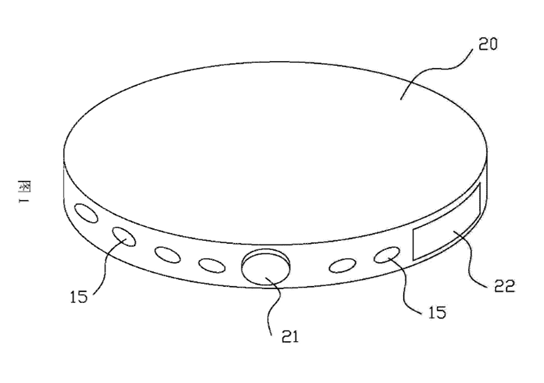
\includegraphics[width=0.5\linewidth]{IP1.png}
    \caption{Intelligent cup coaster (CN204467705U)}
    \label{fig:CN}
\end{figure}

Another device, the \textit{Smart T-caster} (Fig.\ref{fig:IP2}) \cite{IP2} also tries to solve the problem of people forgetting to drink. Again it is an object that is set on a table and not transportable but is connected to a smartphone application in order to track the water consumption. The critical point of this patent is the fact that it is connected remotely to an application on the smartphone that displays information to the user. In the case of "Think Water", the product is different because the water consumption tracking is done on the base system that is physical and in the house, not on an online software accessible remotely. This allows for a more compact coaster in the case of the proposed product.
\begin{figure}[H]
    \centering
    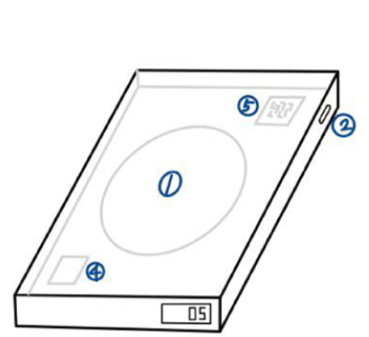
\includegraphics[width=0.4\linewidth]{IP2.png}
    \caption{Smart T-caster (KR20220111927A)}
    \label{fig:IP2}
\end{figure}

A \textit{Drinking Reminder System} (Fig.\ref{fig:IP3}) \cite{IP3} is attached at the bottom of a glass and based on a customized timer, reminds people to drink at regular intervals. This system is basic and not highly personalized which is significant different from the proposed device. It is connected at the bottom of the glass, similarly to what was designed in the product, but it only serves as a drinking reminder. It doesn't perform any measurement of the actual consumption. In the Think Water product,the water intake is tracked and the product reacts accordingly, not solely based on a personalized timer. A regressive model that is specific and personal to each customer is used. From this the system defines a consumption target and react accordingly. The proposed product is not solely meant as a drink reminder, but also sets a consumption target which is really different from this patent.
\begin{figure}[H]
    \centering
    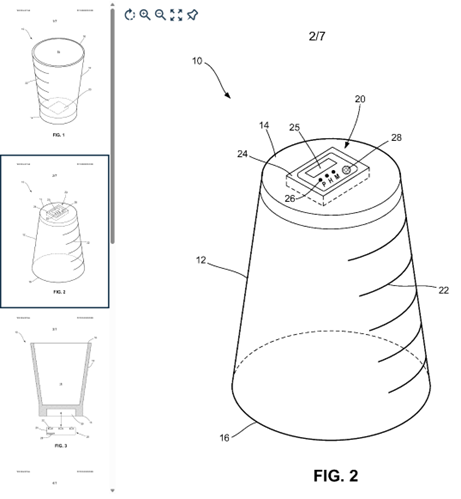
\includegraphics[width=0.4\linewidth]{IP3.png}
    \caption{Drinking Reminder System (WO2016007464A1}
    \label{fig:IP3}
\end{figure}

On the more global view, there is also a patent about the idea and system of drinking reminders working principle (Fig.\ref{fig:IP4}) \cite{IP4}. It states that the global system is decomposed between a measurement device and a central unit processing device, which is very similar to what is proposed. However, this patent expects the measurement module to also do the first processing steps, to have a storage module, to launch the first reminder and to transmit everything to a server that acts as the central unit. On the other hand the coaster only does the measurement. There is no processing, no storage nor decision steps. Everything is transmitted to a physical base that acts as the central unit of the product. This is where all the decision and processing steps will be made. Reminders from the coaster will only be done when asked so by the base. Moreover, they rely on an online server whereas Think Water relies on a physical station present at home to do measurements and set target.
\begin{figure}[H]
    \centering
    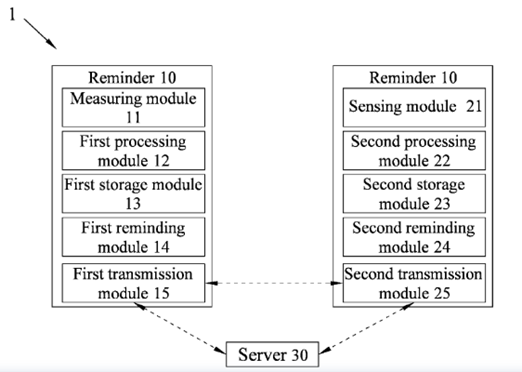
\includegraphics[width=0.5\linewidth]{IP4.png}
    \caption{Drinking reminders working principle (EP 2696302 A2)}
    \label{fig:IP4}
\end{figure}

There are also other similar known products, such as the Droplet Intelligent Hydration Kit from \textit{ALISS}. It is a station that reminds people to drink via audio stimuli \cite{IP5}. However it is designed for people suffering from dementia meaning it is not exactly the same market as the one targeted by Think Water. Also existing is a smart cup  from \textit{Droplet} \cite{IP6}, that tracks hydration level and reminds to drink using flashing lights integrated in the device.  However those 2 device operate alone and don’t require additional systems or devices. It is similar to what is proposed by the product, but not as a whole. The proposed product consists of 2 separate parts, which are similar to the previously mentioned products, but relying on each other and with different functionalities and roles, which makes the product, in the end, different from those currently existing. It allows to cover a larger operating field and combines 2 important stimuli for people (visual and sound) that are adaptable (intensity, frequency, etc.). Plus it sets personalized targets and allows for visual feedback of the consumption, which is not present in the 2 products mentioned above.

\subsection{Patent Search (freedom to operate)}

After looking into what already exists and is protected, it was observed that there are already a lot of technologies and concepts existing that covers dehydration problems. This means that a strong attention to the product system and functionalities will have to be done when commercializing the product, not to infringe existing patents. Section \ref{PriorArtSearch} points out that a lot of devices with similar functionalities exist, such as:
\begin{itemize}
    \item A smart coaster performing measurement 
    \item A processing unit that measures water intake
    \item Drinking reminders if needed (audio, visual or physical)
    \item Customer feedback, using a digital application or a device-integrated screen
\end{itemize}
So people might think that the overall concept of the Think Water product is a copy and a fusion of these already existing devices. But if observing attentively, those patents always have the same structure and try protect the same key points. However, Think Water tries to have a broader vision and bring something that might be simple but has not been done or mentioned previously. And there are many claims to prove it.\vspace{0.2cm}

First composed of 2 different physical parts: the coaster and the base. All the existing patent are about a physical object doing it all at once or a physical object and a server linked to a digital application. The proposed products aims to have 2 physical component in-house, for easier use, especially for elderly people. This sounds trivial but no such existing devices are yet on the market.\vspace{0.2cm}

Secondly, all the measurement performed are never specified. Customizable timers or simply daily targets were mentioned but they are not personalized and accurate for different customer profile. The proposed product uses a regression model that depends on personal information such as sex, age, weight and external parameters such as humidity and temperature. This is something highly innovative. No product existing mentions personalized goals for customers and this is the strong point of Think Water, that is certainly worth protecting.\vspace{0.2cm}

Finally, most of the patents mention a coaster that is not attachable to the glass. It has to be on a table and customer need to put down their glass on top of it to ensure that measurement happens. The only cases where the device is attached at the bottom of the glass is for reminding the customer to drink and not to perform any measurement. In the case of the Think Water product, the coaster, which measures the water intake, is attached to the glass. This allows to transport the glass everywhere and makes sure that the measurement can happen wherever the customer is in his house. This has not been done before, neither mentioned in the field of water intake measurement. This is again something highly innovative and worth protecting. Because it ensures freedom of use to the customer and is a good marketing point as well.\vspace{0.2cm}

Overall, The emphasize will be on the innovation and uniqueness of the product. This way, Think Water will be able to stand out on the market, even though all the elements are not fully patent.
To recapitulate, the strong and innovative points of the Think Water product are: 
\begin{itemize}
    \item The combination and separation of each module with unique function. The coaster and the base have their unique functions, that can be similar to already existing patents, but the combination of how they are used together is really new. Also the fact that they are 2 physical object is new and worth mentioning.
    \item The measurement unit (coaster) is attachable at the bottom of the glass and thus allowing more freedom of use for the customer. This is also something not existing yet that needs to be emphasized. 
    \item The personalized measurement software. Based on a regression model, the software can adjust daily and for each customer the consumption goal. This is something brand new that has not been done previously. 
\end{itemize} 

Overall there are already many patents we need to take into account but the products brings something new that takes advantage of the existing gaps in patents to create a strong and reliable product that can be protected.


\subsection{Discussion on opportunities for IP and possible IP strategy}

Given our product and its specific functionalities we have some IP  ideas to propose:
\begin{itemize}
    \item \textbf{Trade Secret :}
    The regressive model used will be safeguarded as trade secret, ensuring that the model uses the best possible regression for the most accurate prediction and personalization of the goal. It will simply be  mentioned that the product is personalizable, this way, it makes sure that people will not have access to the same regression model the one used by "Think Water".
    \item \textbf{Trademarks :}
    A trademark for the brand name "Think Water" needs to be registered, the logo (Fig.\ref{fig:logogo}) and all associated branding features. The shape and color used will be protected such that Think Water is recognizable and unique. This would ensure distinguishable identity of the product and thus ensuring a stronger impact on the market and the consumer’s mind. It is also a strong sign for the competition that Think Water are serious and invested in the product and on the market.
    \item \textbf{Copyrights :}
    Copyright of the software to make it even stronger and ensure the uniqueness of our product should be done. This regroups the data treatment, how the data are calculated and processed and which data will be collect. The stimuli periods, how often a reminder is sent to the customer and how do the period is determined. The stimuli pattern of the light and the buzzer, meaning blinking lights on the coaster at a specific frequency and on/off buzzing at a specific period on the base and also how the pattern of the stimuli was chosen. This way a really unique product could be achieved by at the same time preventing any copies of it.
    \item \textbf{Patents :}
    Three main claims are to be made, that should ensure that the product is unique and covers enough such that it cannot be copied or replicated easily.\vspace{0.2cm}
   
    As mentioned, the fact that the water intake daily target is personalizable is critical in the product we propose. We could ensure, by patenting the idea, that no other device could perform highly personalizable measurement and set goals accordingly. Meaning that any kind of non-generic settings of daily consumption goal will fall under the patent claim. \vspace{0.2cm}
    
    Attaching measurement unit to the glass through a simple gesture should be protected as well. Including bottles or any object used to drink, to ensure better protection. This is new and an USP of the product, meaning it is a functionality worth protecting. Trying to patent the consept of regrouping different mechanism such as: magnetic, suction, glue, etc, should be done as well. This way, it makes sure that people are not taking advantage of a weak patent.\vspace{0.2cm}
    
    Finally, the device in its integrality should be patented. Using two different complementary and specific modules. Trying to protect the use of a measurement unit and a central unit that are both physically present at the customer's place is important. This would allow Think Water to make sure that if someone wants to make a product that is competitive to Think Water, they will have to find new ideas. The patent should be generic enough in the design such that people cannot simply copy the product but with a different shape. This will be a great success because having a product like the one proposed by Think Water will then be impossible and, as mentioned previously, there are already existing patents if using simply a measurement unit and processing device all in one or if using a measurement unit and a server/digital backup. This way, it will ensure a strong position on the market. Please refer to the \hyperref[appendix:FirstClaim]{first claim} for the list of first claims.
    \item \textbf{Market-specific Adaptation :}
    In the future, the product should be able to be recommended or be used by doctors, it will have to be ensured that the products fits in the health regulations and requirements. adaptations can thus be made to the product to reach this specificities and it would allow for strong marketing arguments and a trusted product that could be recommended by healthcare professionals.

\end{itemize}

Overall the strategy will be divided into different goals and steps for IP in order to ensure uniqueness of the proposed product, to protect it from illegal copying and allow unique feature on the product and Think Water company, to get the maximum from the targeted market.




% ============================================================
% IV. ASPECTS OF A PRE-BUSINESS PLAN
% ============================================================
\section{Aspects of a pre-business plan }
\subsection{Target Demographics}
According to the OFS, people over 65 represented 19.6\% of the Swiss population in 2023 \cite{age}, a figure increasing by 2.3\% annually \cite{swissinfo}. Based on ETH data \cite{ETH} and OFS demographics \cite{OFS}, it is estimated that approximately \textbf{1.54 million} seniors currently live independently without assistance.

International meta-analyses indicate that roughly \textbf{19\%} of people over 65 suffer from dehydration \cite{PubMed}. Applied to Switzerland, this suggests over \textbf{300'000} seniors are at risk annually. This issue is projected to worsen as the senior population reaches 33\% by 2060 \cite{OFS_oldpop}, compounded by rising temperatures due to climate change.

Existing solutions are predominantly designed for institutional settings (hospitals, retirement homes), resulting in bulky and complex devices. A distinct gap exists for user-friendly, non-stigmatizing products tailored for domestic use by independent seniors.\\

The proposed product addresses this gap by enabling seniors to visualize water consumption while offering optional oversight for caregivers. Although not currently medical-grade, the device aims for high accuracy to assist healthcare professionals in diagnosing dehydration as an aggravating factor in hospitalizations.

While the primary market is elderly, secondary markets include:
\begin{itemize}
    \item Health enthusiasts and athletes monitoring hydration.
    \item Families managing children's water consumption.
\end{itemize}

The Serviceable Available Market (SAM) in Switzerland is estimated at \textbf{15'000'000 CHF} (see Section \ref{subsec:finance}). These statistics are transposable to the European level, where the remote patient monitoring market is projected to reach \$1.7 billion by 2025 \cite{EuropeanMarket}.

\subsubsection{Insights from Research}
Surveys \cite{Poll} and expert \hyperref[appendix:interview]{interviews} reveal a dichotomy: while the public perceives dehydration as a minor issue, medical professionals confirm it frequently complicates patient care. Respondents expressed a clear preference for discreet, connected, and simple devices—confirming the viability of the proposed solution.

\subsection{Commercialization Strategy}
Our market entry strategy is structured in two distinct phases to ensure financial stability and rapid adoption.

\textbf{Phase 1: Institutional Validation and Funding.}
The initial commercial focus targets local retirement homes (EMS) alongside a seed funding round from private investors. While EMS contracts provide essential B2B validation and pilot revenue, external investment is required to finance initial inventory and hardware manufacturing setup before achieving scale.

\textbf{Phase 2: Consumer Expansion (B2C).}
Leveraging the credibility and capital gained from EMS partnerships, the strategy will pivot to the core market: independent seniors. At this stage, the product will be introduced to pharmacies and other channels accessible to both seniors and their relatives (e.g., online market). Marketing will highlight the device's success in professional care settings to build trust with families and users. Two tiers will be offered:
\begin{itemize}
    \item \textbf{Basic Version:} A standalone coaster for personal tracking.
    \item \textbf{Advanced Version:} Includes a subscription for remote data access (e.g., for doctors or family).
\end{itemize}
\subsection{Organization}

"Think Water" operates as a specialized med-tech startup driven by a multidisciplinary team of five founders, united by the motivation to bridge the gap between institutional care and independent living.

Project leadership is held by \textbf{Mostafa}, who directs the company's strategic vision and external communications. The technical infrastructure is managed by \textbf{Roméo}, the lead software and electronics engineer. His expertise in full-stack development and electronics assembly allows him to bridge the gap between hardware and software as well as advising other team members.

The physical product design is driven by \textbf{Eliot and Martin}, who oversee mechanical engineering. Their combined proficiency in CAD and rapid prototyping (3D printing, laser cutting) enables the team to iterate quickly and produce functional, aesthetic housings and continuously improve the product.

Finally, market viability is secured by \textbf{Mathieu}, head of business strategy, who manages intellectual property, financial planning, and customer discovery to ensure the product meets genuine market needs. This structure ensures that "Think Water" covers every critical aspect of the product lifecycle, from engineering to business execution.

\subsection{Planning}
\label{FinalProduct}
The development and expansion plan follows a phased approach to manage risk and ensure product readiness:

\begin{enumerate}
    \item \textbf{Pre-Validation:} Before approaching institutional partners, the device undergoes a rigorous internal testing phase. The objective is to identify and rectify major mechanical constraints and software bugs. This ensures the delivery of a stable "Minimum Viable Product" (MVP) to facilitate investor demonstrations and secure initial capital.
    
    \item \textbf{Strategic EMS Partnerships:}Supported by initial investor funding, the priority shifts to signing contracts with local EMS. These partnerships act as a strategic lever to validate the product in a professional setting, de-risking the project for subsequent investment rounds.
    
    \item \textbf{Pilot and Medical Grade Iteration:} Leveraging the EMS access, the product enters a pilot phase to gather user data and refine the hydration algorithms. The long-term goal here is to achieve medical-grade certification, which significantly increases the product's value proposition.
    
    \item \textbf{Swiss Consumer Launch:} Once funded and validated, the product will launch in the Swiss consumer market (pharmacies and online retail), targeting the projected 5\% Serviceable Obtainable Market (SOM).
    
    \item \textbf{European Expansion:} The final phase involves scaling manufacturing to address the \$1.7 billion European market and adapting the software for broader demographics, such as athletes or children.
\end{enumerate}

\subsection{SWOT Analysis}
\begin{center}
\begin{tabular}{|p{0.45\linewidth}|p{0.45\linewidth}|}
\hline
\textbf{Strengths} & \textbf{Weaknesses} \\
\hline
- Adaptable and ergonomic design \newline - Personalized objectives \newline - Optimized for domestic use & - Requires user setup/preparation \newline - Measurement constraints \newline \\
\hline
\textbf{Opportunities} & \textbf{Threats} \\
\hline
- International market access \newline - Demographic trends (aging/climate) \newline - Expansion to new customer bases & - Market competition \newline - Emerging medical alternatives \newline - Low-cost substitutes \\
\hline
\end{tabular}
\end{center}

\subsection{Pricing and Competition}
\label{subsec:finance}

The competitive landscape includes both direct technological solutions and the "status quo."

\textbf{Direct Competitors :}
\begin{itemize}
    \item \textit{H2O-Pal} (\$99): A smart bottle with a connected app. \cite{H2OPal}
    \item \textit{Droplet} (£65): A hydration kit with visual and voice reminders. \cite{Droplet}
    \item \textit{Ulla} (20 CHF): A vibration attachment for bottles. \cite{Ulla}
    \item \textit{TrueLoo} (\$180/year): A subscription-based smart toilet seat for high-end monitoring. \cite{TrueLoo}
\end{itemize}

\textbf{The "Do-Nothing" Competitor}\vspace{0.2cm}

A significant portion of the market relies on the status quo: assuming thirst is a sufficient indicator or relying on memory. While this "competitor" is free, it is inherently risky for seniors, whose thirst sensation diminishes with age. Our product positions itself as a necessary safety net, transforming hydration from a passive assumption into an active, managed metric. To successfully overcome the inertia of this "do-nothing" approach, the product prioritizes optimized user interface experience. By replacing complex setups with a discreet, automated measurement, the device removes the cognitive burden and technical barriers that often lead to technology abandonment among elderly users.\vspace{0.2cm}

\textbf{Market Valuation and Strategy Impact}\vspace{0.2cm}

Positioning the device at \textbf{85 CHF} ($\approx$ x3 production price) places it competitively in the mid-range—more capable than simple reminders like \textit{Ulla}, but significantly more affordable and less invasive than solutions like \textit{TrueLoo}.

Reaching financial sustainability requires rapid volume. The dual strategy of securing EMS contracts and securing early-stage investment significantly de-risks the initial launch. Investor capital will fund the transition from prototype to industrial production, while institutional volume acts as the catalyst for achieving a Serviceable Obtainable Market (SOM) of \textbf{5\%} within the target demographic. While the total Serviceable Available Market (SAM) is valued at roughly \textbf{25'500'000 CHF} (300'000 users at 85 CHF), the SOM is 1'275'000 CHF. Beyond hardware, the recurring subscription model for the "Advanced" version will drive long-term revenue growth and sustainable market expansion.

%---------------------------ANCIEN-----------------
% \section{Aspects of a pre-business plan}

% \subsection{Market}

% According to the OFS, in 2023, in Switzerland, people over 65 years represent 19.6\% of the Swiss population \cite{age} increasing by 2.3\% each year \cite{swissinfo}. This is around 1.73 millions people. Using the numbers from an ETH study \cite{ETH} and graph from OFS \cite{OFS}, we estimated an overall number of people over 65 living in a house without assistance to be around \textbf{1.54 million}.\vspace{0.2cm}

% Since our problem is concerning dehydration, we needed to check what percentage of people were affected by dehydration. Finding a specific paper about Switzerland is quite complicated. But on a larger scale, we can find studies that are serious enough such that we can extract information and apply them to Switzerland. We used an international meta-analysis by PubMed that states that the amount of people over 65 suffering from dehydration is around \textbf{19\%} \cite{PubMed}. This gives us over \textbf{300'000} seniors subject to dehydration every year.\vspace{0.2cm}

% This issue is expected to grow and become more problematic in the next the years. According to the Swiss Federal Statistical Office (OFS), the part of the population over 65 years old is expected to rise and reach 33\% by 2060 \cite{OFS_oldpop}. Combined with the effects of climate change, which increases dehydration risks, the problem is set to worsen in the coming decades. This trends indicate a growing problem which need to be solved, in Switzerland, and worldwide.\vspace{0.2cm}

% Existing hydration-monitoring solutions are mainly designed for institutional environments such as hospitals or retirement homes and are often bulky and complex.
% There are no widely available, user-friendly products tailored for domestic use, particularly for seniors living independently. That why we prioritize this target.\vspace{0.2cm}

% Our goal is to offer a product that could fill the gap. It is primary for elderly people living at home. Helping them to visualization their water consumption and could also be used by nurses or family to check if the elderly person is drinking enough according to the recommendation.\vspace{0.2cm}

% It is important to note that our device is not medical grade. We however want to make something accurate such that it can be recommended by healthcare professionals. Because after some interviews we conducted with doctors, when someone gets hospitalized, it is often hard to determine if the reason is dehydration but it is for sure an aggravating factor. By making an accurate enough product, doctors could use the data to determine faster if dehydration is a factor or not.\vspace{0.2cm}

% Note that the primary market is already wide but could be extend in the future to:
% \begin{itemize}
%     \item {Health enthusiasts that want to monitor their water consumption}
%     \item {Athletes that need to be very cautious on their hydration level}
%     \item {Families that want to control their children water consumption}
% \end{itemize}\vspace{0.2cm}

% Overall, the serviceable available market (SAM) as a value of \textbf{15'000'000 CHF} (see section \ref{subsec:finance}), solely in Switzerland. All the statistics are are transposable to the European level, due to the similar development in those countries. In Europe, remote patient monitoring market cap is 1.6 billion \$ in 2025 \cite{cap}. 

% \subsubsection{Insights from research and interviews}

% Through extensive search, polls \cite{Poll} and expert \hyperref[appendix:interview]{interviews}, we identified several key insights:
% \begin{itemize}
%     \item Public perception: The majority of people surveyed believe dehydration is not a major problem in Switzerland.
%     \item Medical perspective: Doctors, however, report that dehydration is often a secondary diagnosis, if not primary, in hospitalization that complicates patient care. 
%     \item Vulnerable groups: Unanimously, seniors are the most exposed, especially those affected by medical treatments, disabilities, or psychological illnesses.
% \end{itemize}\vspace{0.2cm}

% These statements confirm and reinforce the national statistics and the need for prevention. This is why we think our product has good chances of success. Because of a actual need and a significant and growing market.\vspace{0.2cm}

% When asked what kind of solution they would prefer, most respondents expressed interest in a connected, discreet, and easy-to-use personal device that could monitor hydration levels and issue alerts when necessary.\vspace{0.2cm}

% However, no satisfactory device currently exists for elderly people living at home or in apartments — representing a clear market opportunity.\vspace{0.2cm}

% \subsection{Strategy towards commercialization}

% Our product is a personal hydration monitoring product which is easy to use and not invasive. This allows to use such a product at home without any assistance. Also, the consumption objectives are personalized for each users. Our product is distinct from the competitors due to these key features which will drive our marketing. The idea is to showcase them and use them to attract a large number of customers.\vspace{0.2cm} 

% We will offer 2 different versions of our product. The basic one and the advanced one.
% The basic one consists of the coaster and the base, working together as we described. This is the most interesting one for people who are reticent to share data online or allow remote access. All the functionalities are the same and ensure precise measurement and specific daily goals for each users with consumption tracking and display over several month. This basic option ensures that the product will generates some revenues due to its functionalities and reasonable cost.\vspace{0.2cm}
% The advanced version requires, additionally to buying the product, a monthly subscription. This is because not only it works as the basic one, but we ensure external communications and remote access to the data. This would allow families or doctors to access those data. It could be really helpful in the case of people who are more isolated or more at risk and provides also a way for the family to check actually on their elder's water consumption, making sure that this is not a problem for them. This is more costly but the price difference and the impact our product could have will encourage people who can afford it, to buy it. This will generate dynamic income and enable us to ameliorate our product even further.\vspace{0.2cm}
% Regarding the software, we could think of some updates adding additional features if needed. We could make them free for the people owning the advanced version but offering a reduce cost for people with basic version if they want to access new features on their product %pas sur mais à discuter ça peut être une bonne idée.

% To enter the market we will rely mainly on advertisement that we will displayed, for example, in pharmacies or targeted locations where elder people tend to gather. We will of course display a people from the targeted audience and try to make our product as discrete as possible on the shot but clearly displaying it on the side. The idea is that the product appears discrete and nice looking such that people are not scared or reticent to buy it, thinking it will not fit in their home. It is also important to minimize the software part in the advertisement such that elderly are not frightened because they think they will not be able to use or understand it. Additional, the idea is to make television advertisement, encouraging the use of our product and focusing on the visual and sound stimuli rather than on the screen display. We should also focus on the domestic use. Proving that our product is discrete, compact and that people coming will not be bothered by it, maybe even on the contrary they will be curious.\vspace{0.2cm}

% To further improve our market introduction, if we achieve medical grade device, we could ask healthcare professionals to recommend our product and also use this grade in our advertisement. This will associate a serious image to our brand and will boost the customers trust in our product. We could also think about partnerships with EMS or insurance companies. Because our product could potentially lower the costs of new patient or hospitalization due to hydration issues. This would again, further increase our image and the strength of our product on the market.\vspace{0.2cm}

% Since our product targets a wide range of people, we would like to make it available in many locations. The primary ones would be pharmacies. Since it is a product that can help water consumption, it would make sense that pharmacies sell it. However we would also like to make it available online such that people can buy it more easily and also such that people could buy it for their elders. We do not need that the elder are the ones buying the product directly. By choosing pharmacies we ensure that people trust our product.\vspace{0.2cm}



% \subsection{Your organization}
% "Think Water" is a company created by 5 talented individuals, each bringing a different yet complementary approach and exceptional dedication to the company.\vspace{0.2cm}

% Mostafa was the manager. He is the one making sure the product is presentable and that the communication with other is done smoothly while serving the company's interests. He was also our dedicated solder, making sure all electronic components are well assembled and connected together.\vspace{0.2cm}

% Roméo was our software engineer and electronical engineer. He took care of the code with unique dedication, pushing its limit such that customers can have the best product available on the market. He came up with a clean user interface and is willing to make it even better in the future. He also was the bridge between the people working on the product. He knew all the components and how to use them and he can guide people on what they have to do and how they should do it.\vspace{0.2cm}

% Eliot and Martin were in charge of the mechanical part of the product. Designing the devices using CAD, printing or laser cutting the different parts required to assemble the final product. Their hard-work and perseverance upon failures and retry was exemplary and lead to a final prototype which was really encouraging. Together they made sure that the 2 products were aesthetically good looking while being functional together.\vspace{0.2cm}

% Mathieu was more focused on the market analysis and IP strategy. He is the one who proposed a patent and first claim. He was the one interviewing people to get as many information as possible on the market in order to adopt the best strategy and best product idea together with the other members. He was also in charge of the finance of the company in order to fit the budget and make sure the product we bought were absolutely necessary for the prototype.\vspace{0.2cm}

% Overall, the team was really complementary and allowed to create a good atmosphere and working space in order to create a really innovative product which has its place on the market.
% % À compléter : structure d'équipe, rôles et compétences nécessaires.

% \subsection{Planning}
% %Probablement ici on peut faire un sous-chapitre ou juste expliquer ici les market opportunities ça serait le plus juste
% To offer a functional product, we will need to make some adjustments. We detailed them in the \nameref{FinalProduct}. We could use a pilot testing in partnerships with EMS such that it is still in a controlled medium in case of issues. This will allows us to get feedback towards a final product, and check the potential possibility to reach medical grade.\vspace{0.2cm}

% Then we will start entering the market. Using strong and targeted advertisement, first in Switzerland. For this we will need to establish scaling manufacturing capacities such that we can follow the demand for our product. Also, we will need to have retailers that accept to sell our product, this will have to be negociated before entering the market.\vspace{0.2cm}

% Once the initial market is set and stable we can start go European first. This already represents a global market cap of around 1.7 billions \cite{EuropeanMarket}. This would require no change in the product or the advertisement method but will allow for larger income. But we will need to check that the manufacturing process is sufficient for the demand.\vspace{0.2cm}

% Then the final step can be international expansion. Again we have a global market cap that could reach 3.5 billions \cite{InternationalMarket}. This would mean to have strong production capabilities and reviewing IP as well. But it will allow us to go on the international scene which is best for our company development.\vspace{0.2cm}

% Finally if we want to reach larger audience, the product could also be addressed, not only to elderly people, but to any kind of people wanting to track their hydration level and to make sure they drink enough, such as athletes for example. This would not require fundamental changes in our product but it will require different advertisement methods and ensuring that the product we sell fulfills a need from the customers.\vspace{0.2cm}
 
%  We could also think of adaptation of the software such that it is more attracting for children by adding more colors or different light patterns and little animations on the screen. This could also be an interesting market to investigate.
% % À compléter : vision de croissance de la société sur quelques années.

% \subsection{SWOT analysis}

% \begin{center}
% \begin{tabular}{|c|c|}
% \hline
% Strength & Weakness\\
% \hline
% - Adaptable and ergonomic & - Requires to prepare the product \\
% - Personalized hydration objectives & - Constraints to perform accurate measurement \\
% - Specialized for domestic use & -  \\
% \hline 
% Opportunities  & Threats\\
% \hline
% - International market access & - Concurrence \\
% - Can reach more customers & - New medical solution to prevent dehydration \\
% - Climate change and aging population & - Similar product at lower costs\\
% \hline
% \end{tabular}
% \end{center}

% \subsection{Pricing analysis / competition}
% \label{subsec:finance}

% The existing device that enter in competition with our product all have different prices and billing systems.
% \begin{itemize}
%     \item\textit{H2O-Pal} sells a smart bottle, with a connected software that monitors the water consumption and displays monthly evolution. All of this for 99\$. \cite{H2OPal}
%     \item \textit{Spearmark Health Ltd} offer a Droplet Intelligent Hydration Kit, consisting of box sending visual and pre-recorded voice signals to remind the person to drink. It is available at 65£. \cite{Droplet}
%     \item \textbf{Ulla} has a bottle attachment that vibrates and reminds you when you don't drink enough. Their selling price is 20 CHF. \cite{Ulla} \cite{SmartGlass}
%     \item \textbf{TrueLoo} sells a toilet seat with optical sensors that measure the water concentration in urine and can determine the hydration of the person. It is also equipped with a software to access the data and visualize the consumption of water over some periods of time. The format is a monthly subscription for 15\$, leading to a yearly bill of 180\$. \cite{TrueLoo}
% \end{itemize}\vspace{0.2cm}

% Overall, the market we are targeting represents around 300'000 people. If we want to sell our device 50CHF, which is, when looking at what the concurrence offers as product and considering our USP, reasonable. It will be in the middle of the price-spectrum of hydration device but will guarantee precise measurement,personalized target and allow domestic use without strong restrictions.
% Moreover, the device doesn't require any external maintenance because everything is stored locally. We could maybe add a monthly fee for those who want to have access online to their data for personal use or to share with doctors and other professionals. This fee could be up to \textbf{10CHF} monthly which makes it reasonable.\vspace{0.2cm}

% If we want to estimate our market value, we could assume a conversion rate of 5\%. This estimation of the conversion rate is determined from a poll we made. In the pole, one of the question was \textit{Would you be ready to invest in this project?} We obtained a \textit{Yes/Yes, depends on the price} higher than 50\% \cite{Poll}. This is why we are confident to assume this conversion rate of 50\%.
% With all these consideration, we could reach a market value of around \textbf{15'000'000 CHF}. 

% This format ensures competitive positioning on the market as well as delivering a complete system to track hydration with customized goals and prevent dehydration problems while also ensuring a value we could take profit of.

\section{Project Management}

\subsection{General Strategy}
The team was naturally split based on people's best interest. We all did globally the market analysis together and some members continued in accord to the MS2 feedback thus allowing the team to work more on the prototype. \vspace{0.2cm}

The design and functionalities of the device were subject of great divergences but we all ended up agreeing on what was best and achievable by discussion and grading proposition on defined criterias. When we started the design part, since our product was decomposed in two physical objects, two people worked on the CAD and design separately while still communicating. The two others were in charge of the electronics and finding the components we needed for the prototype.\vspace{0.2cm}

After this step, one member fully dedicated its time to the software. This allowed us, using the weekly meeting and also meeting out of the class, to advance at a nice speed and ensuring everybody was keeping up and had something useful to do. \vspace{0.2cm}

We had to exchange and communicate a lot since all the parts were taken care of by different individuals. We thus set clear objectives for each meeting and making sure everyone was at the same point each time we met. This allowed us to have a final prototype ready by the time of the final presentation.\vspace{0.2cm}

When coming to the end the people who finished their tasks early were assigned to the report and final presentation and slides. This ensured good and coherent presentation quality while being able to finish the prototype without rushing and risking catastrophic failures.

\subsection{Work breakdown structure}

The Work Breakdown Structure (WBS) used during the project is shown in Figure \ref{fig:WBS} (next page).

\begin{figure}[H]
    \hspace{-0.8cm}
    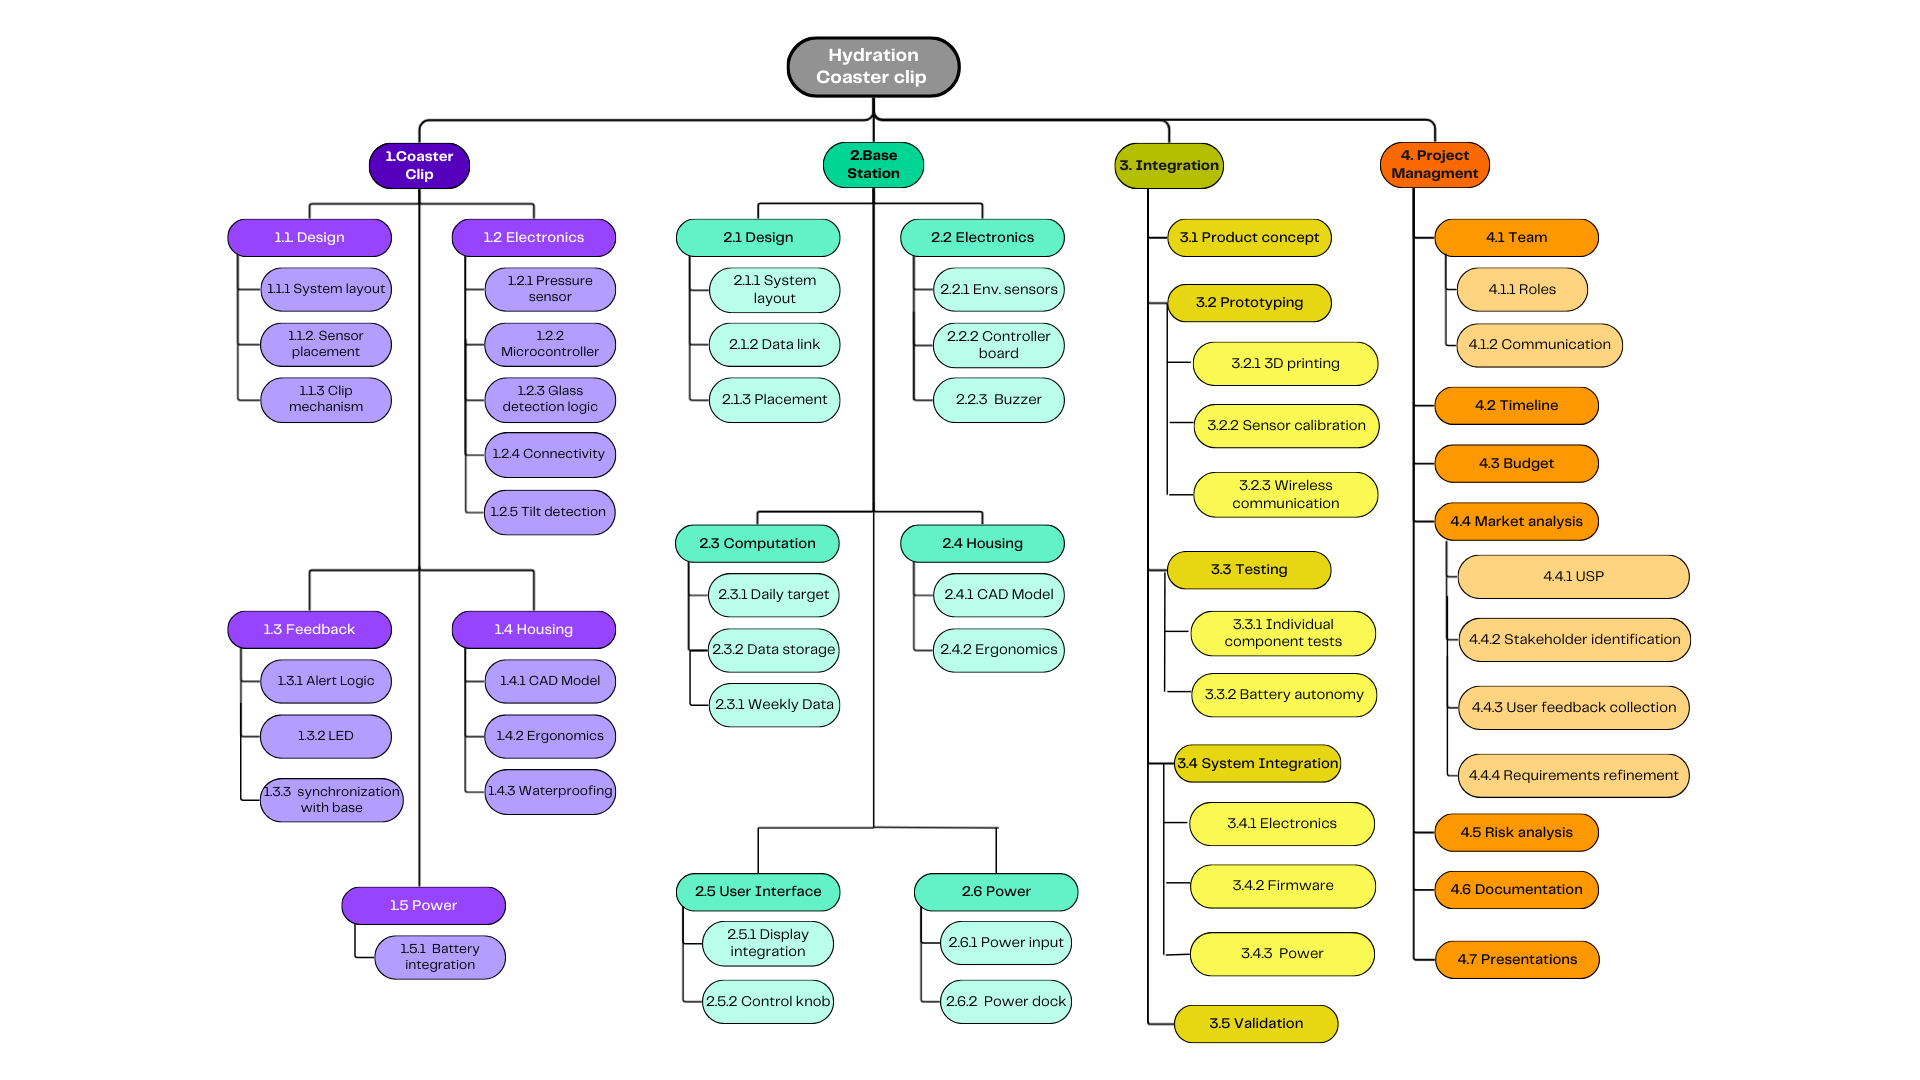
\includegraphics[trim=3cm 0cm 2cm 1cm, clip,width=0.8\paperwidth]{logos/wbs.png}
    \caption{Work Breakdown Structure diagram for the "Think Water" project.}
    \label{fig:WBS}
\end{figure}

\subsection{Stakeholder analysis}

The stakeholder analysis is summarized in the following figures.

\begin{figure}[H]
    \hspace{-0.5cm}
    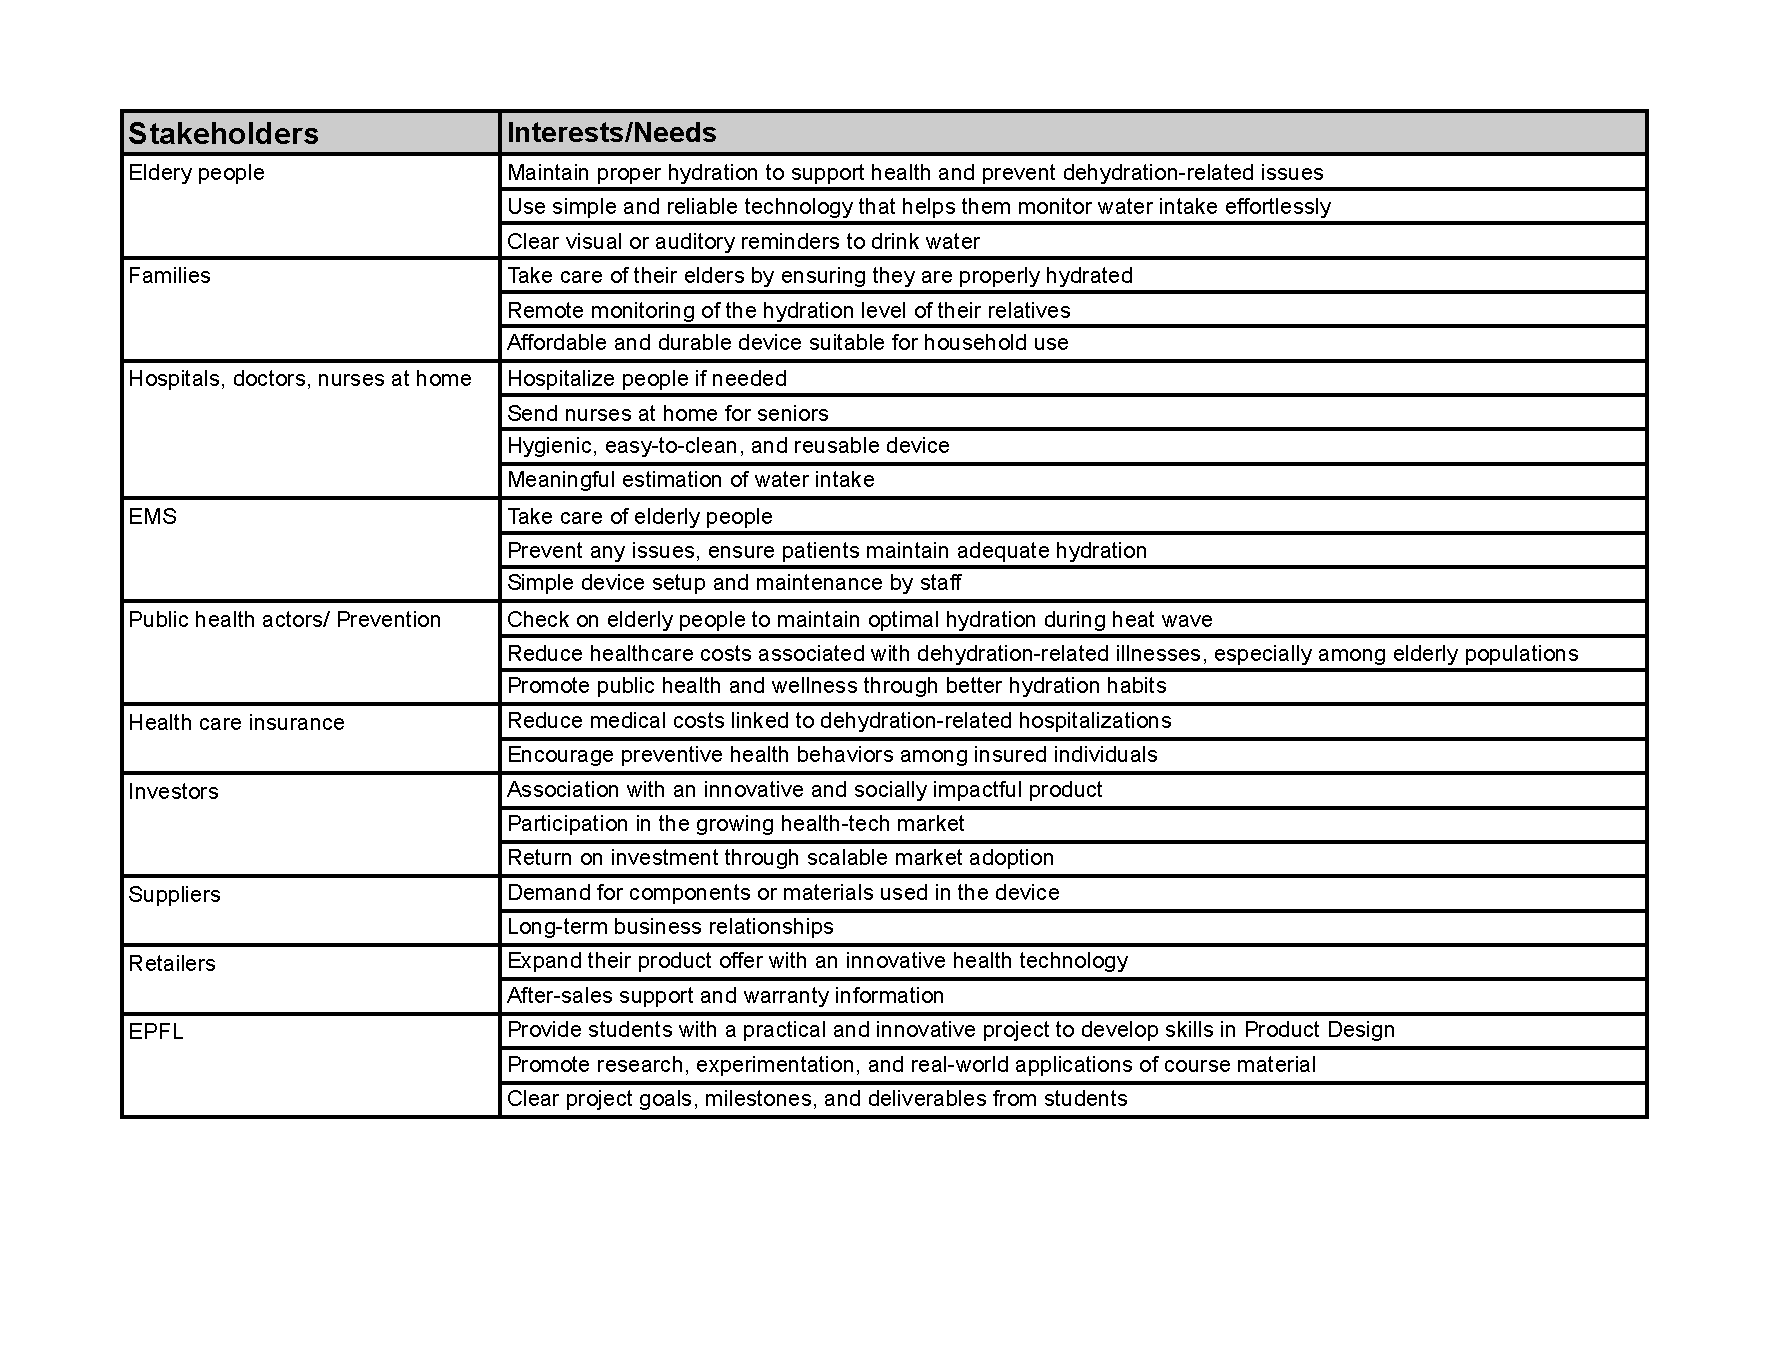
\includegraphics[trim=2cm 3.9cm 1cm 1.8cm, clip, width=0.8\paperwidth]{logos/Table of stakeholders.pdf}
    \caption{Stakeholders and their interests/needs.}
\end{figure}


\begin{figure}[H]
    \centering
    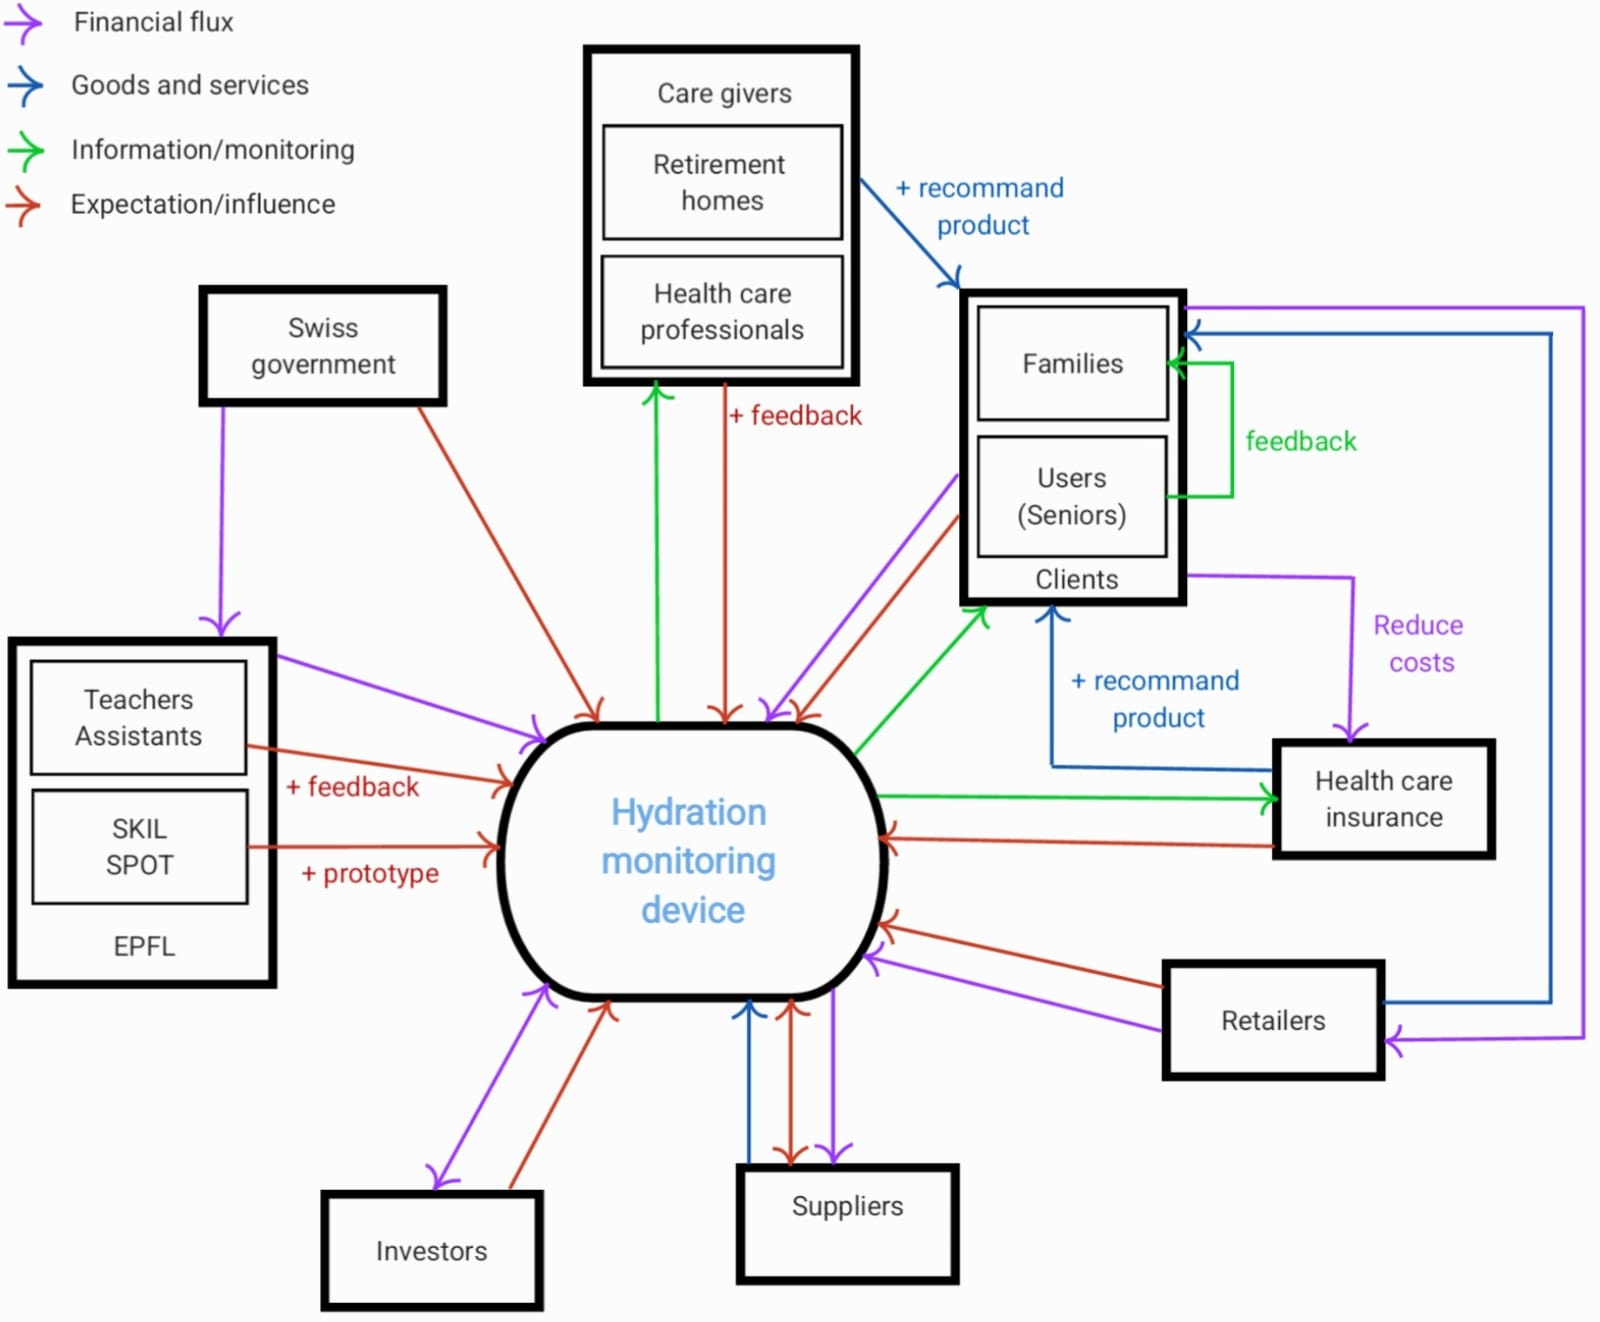
\includegraphics[width=0.95\textwidth, trim=0cm 0cm 0cm 0cm, clip]{logos/stackholder graph new.jpeg}
    \caption{Stakeholders and their relations graph.}
\end{figure}


\subsection{Gantt chart}



\subsubsection{Initial plan}

The Gantt chart (Fig.\ref{fig:gantt}) describing the planning of the project is shown below.

\begin{figure}[H]
    %\centering
    \hspace{-1.1cm}
    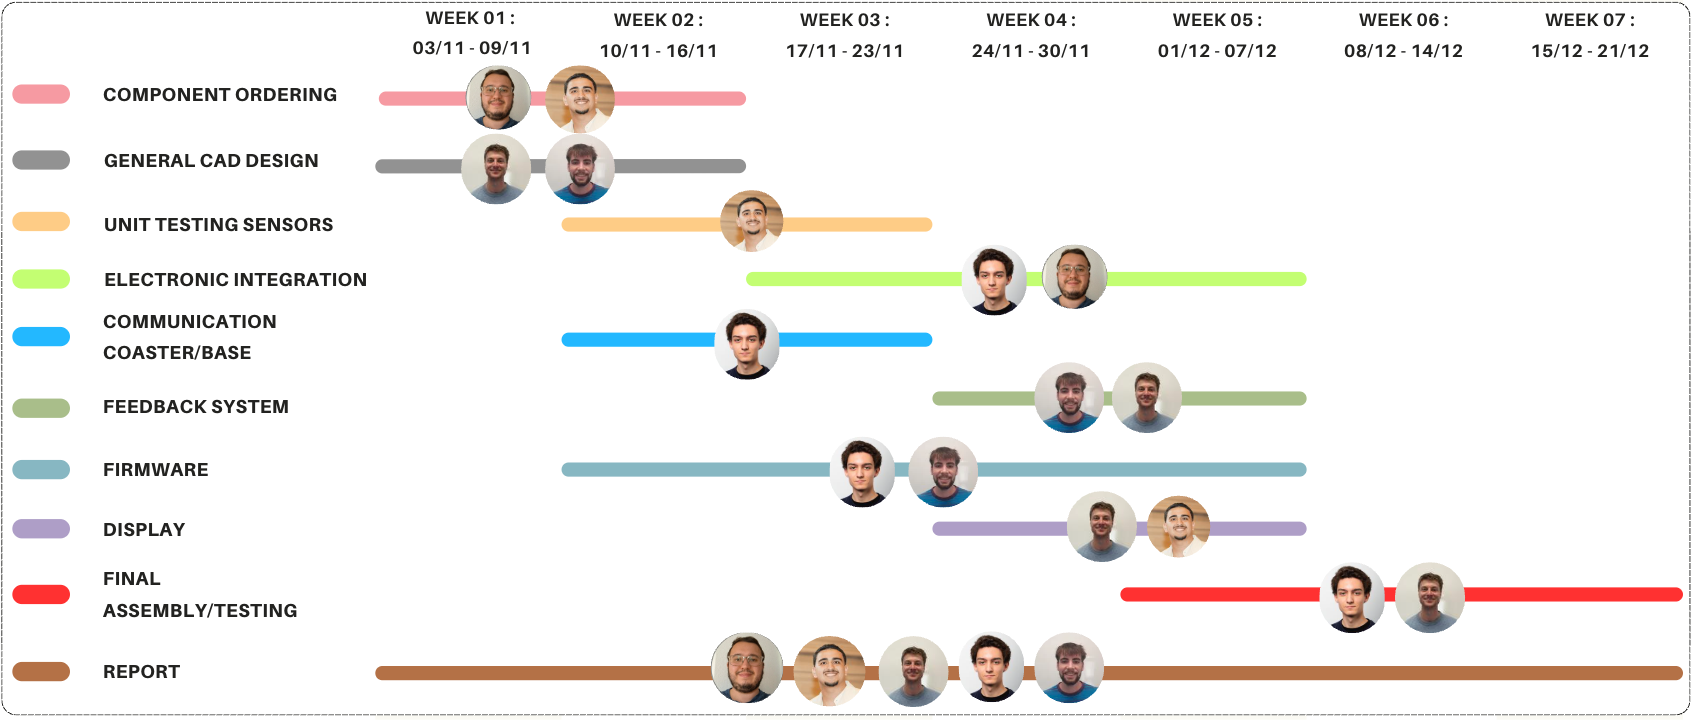
\includegraphics[width=0.85\paperwidth]{logos/gantt.png}
    \caption{Project Gantt chart.}
    \label{fig:gantt}
\end{figure}
\newpage
\subsubsection{Deviation from the original planning}

Overall, the project followed the initial planning presented in the Gantt chart, but several tasks required more time than originally anticipated. In particular, component delivery took longer than expected due to supplier delays, which postponed the start of electronic integration and limited early hardware testing. To cope with this, we temporarily shifted the focus toward CAD design, firmware development, and unit testing using available components.\vspace{0.2cm}

Additionally, the integration and calibration of sensors proved more time-consuming than planned, especially for the load cell and multi-sensor fusion logic. This required extra iterations to ensure reliable measurements in real-life conditions. As a result, some tasks such as communication and feedback system development partially overlapped instead of being strictly sequential.\vspace{0.2cm}

To mitigate these delays, tasks were reallocated among team members, allowing parallel work on firmware, mechanical design, and report writing. This flexible redistribution of resources helped maintain steady progress and ensured that final assembly, testing, and documentation were completed on time despite the deviations from the initial schedule.


\subsubsection{Reflection on how the project went}

Throughout the project, we encountered several challenges, mainly related to technical integration, manufacturing constraints, and time management. On the technical side, combining multiple sensors into a reliable drinking detection system required more iterations than expected, especially during calibration and real-life testing. Manufacturing-wise, assembling compact electronics inside the coaster and ensuring mechanical robustness demanded attention to details to reduce prototyping cycles (only 3 print for the coaster and 0 cycle for the base).\vspace{0.2cm}

From a managerial perspective, coordinating parallel tasks such as hardware development, firmware implementation, and documentation required careful planning. To address these challenges, we maintained regular communication within the team, redistributed tasks when needed, and adapted the schedule dynamically. Overall, the team remained well organized and reactive, which allowed us to overcome difficulties efficiently and deliver a functional and coherent prototype.

\subsection{Who did what?}
\textbf{Mathieu} - My main contributions on the project were for the market analysis and the IP study. I went to talk to doctors to get some feedback on the market we were interested in. I also looked up the numbers and check on the market trend and evolution to see if a product could fit in there. I also checked on the concurrence to make sure we were doing something new and innovative. Regarding the IP study, it was in the following of the market and concurrence analysis and study. Since I already done the most research about the subject it was logical that I continued in this way.  I was able to read and check what was existing and protected and to find the gaps where our product could fit and how to protect it as well. Finally as everyone I took part in the discussion regarding the design, functionalities and implementation of the final product. I helped with the creation of the base mostly and some hands here and there when needed. I think I did more of a non-engineer work but this allowed the team to focus more on the prototype and for me to learn new soft-skills. This was then interesting to me and helpful for the team.\vspace{0.2cm}

\textbf{Mostafa} - As the project manager, I was responsible for ensuring that the project progressed smoothly and that the final product was presentable and coherent. I coordinated communication within the team and with external contributors, making sure that decisions served both the technical objectives and the overall vision of the project. I was also in charge of welding and electronic assembly, ensuring that all components were correctly integrated, reliably connected, and functional throughout the development and testing phases.\vspace{0.2cm}

\textbf{Eliot} - I mainly focused on the mechanical design of the base station. I spent a significant amount of time working between SKIL and SPOT to design, prototype, and improve the wooden base using CAD and laser cutting. This iterative process allowed me to refine the structure, ensure proper integration of the electronic components, and achieve a design that is both functional and aesthetically discreet for domestic use. Through multiple trials and adjustments, I contributed to making the base station robust, well-finished, and well integrated with the coaster.\vspace{0.2cm}

\textbf{Martin} - I was primarily responsible for the mechanical design and optimization of the coaster using CAD. I worked extensively at SPOT to prototype, redesign, and resize the coaster through three iterations, focusing on compactness, ergonomics, and fit of components. 3D printing was used for these iterations by testing different geometries and assembly solutions, I improved the reliability of the attachment mechanism and the overall robustness of the coaster. My work ensured that the coaster remained discreet, functional, and well adapted to everyday domestic use. Concerning the report, I did the stakeholders graph and ConOps and help with the stakeholder interests/need as well as the technical solutions tables (as everyone). I also did the market strategies for the deployment of our product to fit the real world market and finance needs.\vspace{0.2cm}

\textbf{Roméo} - I was in charge of the software and electronic aspects of the project. I developed the firmware architecture, implemented the core logic of the system, and designed a clean and intuitive user interface for the base station. I also ensured proper communication between the coaster and the base, pushing the code to be both efficient and reliable. In addition, I acted as a technical bridge within the team, helping others understand the components, their interactions, and guiding integration decisions throughout the project.

% Chaque membre décrit sa contribution (paragraphe chacun).

%\newpage

% ============================================================
% VI. CONCLUSIONS
% ============================================================
\section{Conclusions}
\label{FinalProduct}
\label{sec:perspective}

This project allowed us to design, prototype, and evaluate an innovative domestic hydration monitoring system aimed at seniors living independently. Overall, the outcome of the project is very positive: we successfully developed a functional prototype that demonstrates the feasibility, relevance, and originality of our product. From a technical perspective, the core functionalities (accurate sip detection, personalized hydration targets, intuitive feedback, and low-power operation) were implemented and validated through real-world testing. From a project management standpoint, the team was able to coordinate mechanical, electronic, and software development efficiently; while having a fun and productive team atmosphere.\vspace{0.1cm}

Nevertheless, several aspects could have been improved. Some phases, particularly manufacturing and component integration, started later than initially planned due to delivery delays, iterative prototyping, and calibration challenges. While these difficulties slowed down progress, they also provided valuable learning opportunities and led to more robust design decisions. In hindsight, earlier validation of suppliers, more buffer time for mechanical iterations could have further optimized the development process.\vspace{0.1cm}

Our prototype represents an important step toward a real product, but several improvements would be required before market launch. On the technical side, some points remain to be refined, such as battery efficiency, further miniaturization of the coaster to make it even less invasive, and optimization of the attachment mechanism between the glass and the coaster. We also identified opportunities to enhance user feedback by combining visual reminders with physical stimuli such as vibration, and to improve usability through a larger, tilted display on the base station. Other important upgrades include wireless charging, richer data visualization, improved glass-change detection, and making the coaster splash-proof or fully waterproof.\vspace{0.1cm}

Beyond purely technical aspects, future developments would also involve strategic decisions. Enabling secure external data access for families or healthcare professionals could significantly increase the product’s impact, but would require careful handling of data security and privacy. Additionally, while the current prototype is not medical-grade, obtaining medical certification in the future could strengthen credibility, allow healthcare professionals to recommend the product, and unlock new funding or reimbursement opportunities.\vspace{0.1cm}

In conclusion, this project demonstrated that a discreet, non-invasive, and personalized hydration monitoring solution for domestic use is both technically feasible and socially relevant. The prototype validated our initial concept and highlighted clear paths for improvement and scaling. Considering the growing aging population and the lack of simple at-home hydration monitoring solutions, we believe this product has strong potential. Given the progress achieved and the clarity of future prospects, we would confidently consider investing further time and resources into transforming this prototype into a real, market-ready product.\vspace{0.6cm}

\centering
    \textbf{And remember with THINK WATER thirst will be a souvenir}
    
\includegraphics[width=0.11\paperwidth]{logos/logo_sans_text.png}



% À compléter : bilan global du projet, ce qui a été atteint, améliorations possibles, perspectives.

\newpage

% ============================================================
% VII. ANNEXES / SUPPORTING DOCUMENTATION
% ============================================================
\appendix
\section{Annexes / supporting documentation}

\subsection{Risk assessment}

This section presents a global risk assessment of the "Think Water", covering both manufacturing risks (MR) and operational-life risks (OR).

\begin{adjustwidth}{-2cm}{-2cm}
\begin{longtable}{|p{1cm}|p{3.2cm}|p{4cm}|c|c|p{4cm}|}

\hline
\rowcolor{blue!25}
\textbf{Code} & \textbf{Risk} & \textbf{Cause} & \textbf{Impact} & \textbf{Likelihood} & \textbf{Mitigation} \\
\hline
\endfirsthead

\hline
\rowcolor{blue!25}
\textbf{Code} & \textbf{Risk} & \textbf{Cause} & \textbf{Impact} & \textbf{Likelihood} & \textbf{Mitigation} \\
\hline
\endhead

\hline
\multicolumn{6}{|r|}{\small Continued on next page} \\
\hline
\endfoot

\hline
\endlastfoot

% ============================
% MANUFACTURING RISKS
% ============================

MR1 & Impossible to assemble & Wrong CAD dimension in relation to component size & High & Low & Iterative 3D printing, include margins for error \\ \hline
MR2 & 3D print structural weakness & Poor design and wrong print parameters & Medium & Medium & Iterative 3D printing, ask for help at SPOT \\ \hline
MR3 & Damaging the electronics during assembly & Human assembly error & High & Low & Assemble with care, preparation and patience \\ \hline
MR4 & Defective components & Supplier issue & High & Low & Incoming quality control and unit test \\ \hline
MR5 & Delay components & Supplier issue (Ali Express) & High & Low & Backup components in Spot and adapt the product or reorder on Digikey \\ \hline
MR6 & Battery failure & Wrong battery usage & High & Low & Use battery with charge/discharge protection circuit, check polarization \\ \hline
MR7 & Poor adhesion of VHB pads & Wrong glass surface or wrong adhesive selection & High & Medium & Test, additional (waterproof) glue if needed \\ \hline
MR8 & Imprecise measurements & Imprecise calibration steps & Medium & Medium & Find more robust way to calibrate \\ \hline
MR9 & Overly sensitive accelerometer & Wrong motion detection threshold & Medium & Low & Adapt the accelerometer and test real life uses to find the right threshold \\ \hline
MR10 & Data loss on SD & Corruption / removal during writing & Medium & Medium & Safe data writing routines, backup storage on microcontroller \\ \hline
MR11 & BLE communication loss & Distance or interference & Medium & High & Local data buffering and reconnection attempts \\ \hline
MR12 & Unexpected product behaviors & Oversight in code logic & High & Medium & Frequent end-to-end testing \\ \hline
MR13 & Poor battery life & Power consumption too high & Medium & Medium & Sleeping mode, minimal communication and sensor activation \\ \hline

% ============================
% USER RISKS
% ============================

OR1 & Power adaptor stops supplying power to base & Defective adapter, power outage, unstable voltage & High & Medium & The controller must be prepared to lose power at any moment, and not lose data \\ \hline
OR2 & Battery overheating & Long exposure to heat & High & Low & Use protected cell, safety warnings \\ \hline
OR3 & Battery wears out & Aging & Medium & Medium & Battery health monitoring and recommendation to replace \\ \hline
OR4 & Water spilling into coaster & No waterproofing / misuse & Medium & High & Waterproof design and usage precautions in user manual \\ \hline
OR5 & Coaster detaches and falls & Weak magnets or glue & Medium & High & Magnet strength validation, VHB surface preparation, shock resistant design and material choice \\ \hline
OR6 & Magnets too strong & Pinch hazard and hard to detach & Low & Low & Limit magnet size/strength \\ \hline
OR7 & User drops coaster & Human error & Medium & High & Mechanical reinforcement, drop tests, material choice \\ \hline
OR8 & User misinterprets alerts & Elderly user difficulty & High & Medium & Simple icons, color codes and short audio patterns \\ \hline
OR9 & User annoyed by buzzer & Noise sensitivity & Low & Medium & Configurable volume or mute option \\ \hline
OR10 & User forgets to charge coaster & Inattention and oversight & Low & High & Low-battery visual signal or alert or message on base screen \\ \hline
OR11 & Incompatible glass shape & Curved or uneven base & Low & Medium & Recommendation of compatible glass shapes \\ \hline
OR12 & Magnet corrosion & Exposure to water & Medium & Low & Use non-corrosive magnets \\ \hline
OR13 & Knob too stiff & Arthritis or low strength & Medium & Low & Low-force rotary encoder \\ \hline

\captionsetup{justification=centering}
\caption{Risk analysis and mitigation strategy for the prototype implementation}
\label{tab:risk_analysis}

\end{longtable}
\end{adjustwidth}



\subsection{Risk matrix}

\begin{figure}[H]
    \centering
    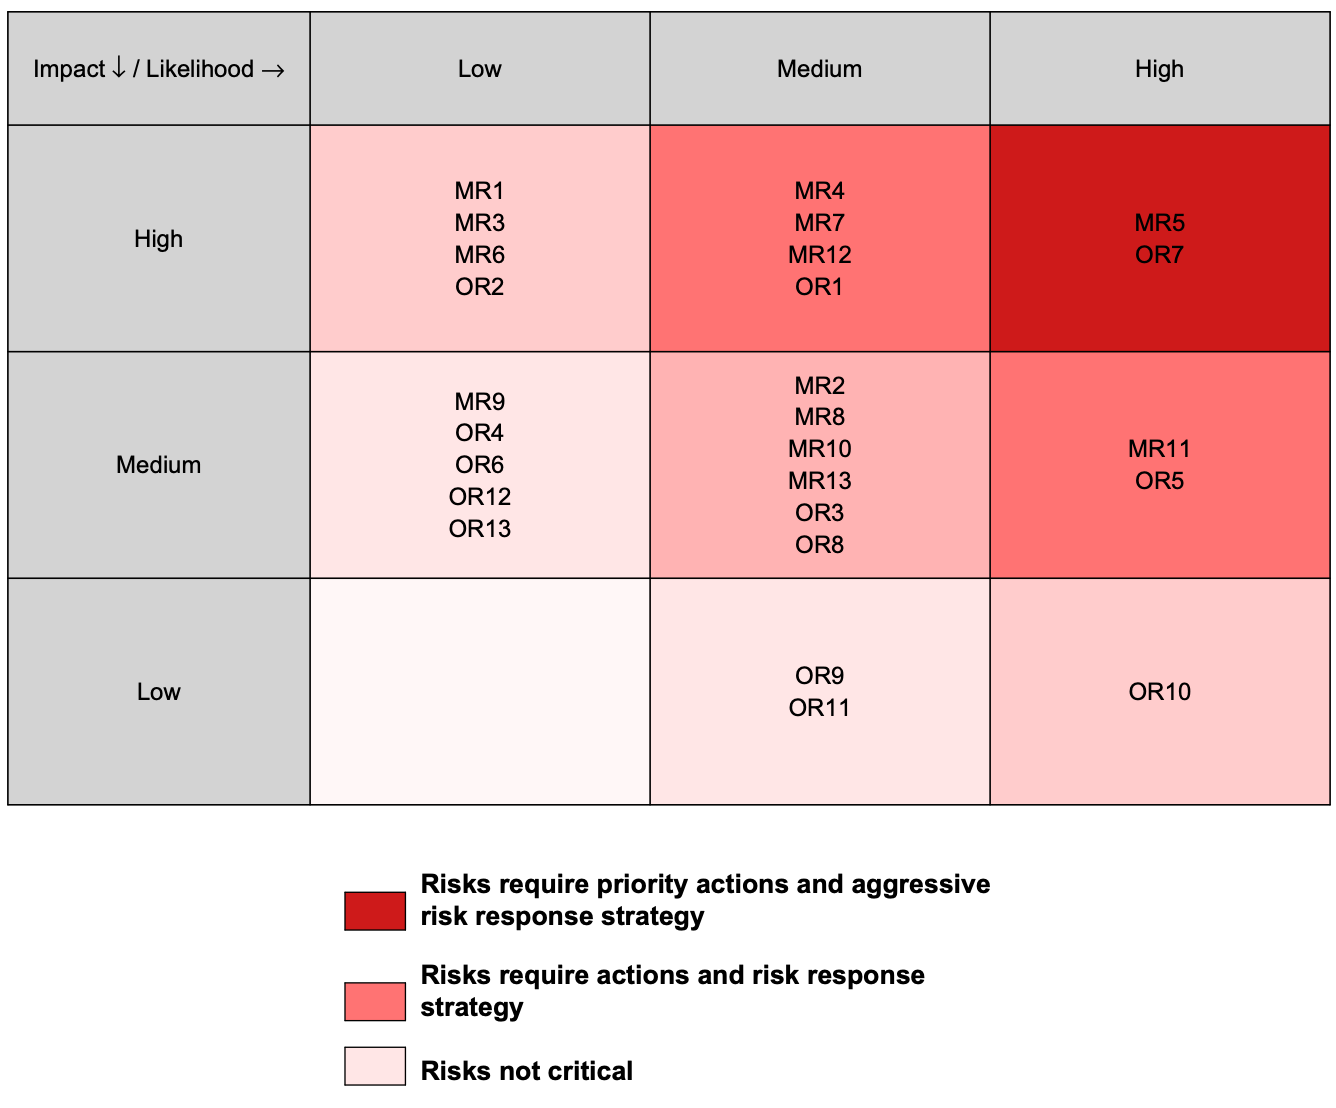
\includegraphics[width=0.8\textwidth]{logos/matrix.png}
    \caption{Risk matrix summarizing impact and likelihood of MR and OR codes.}
\end{figure}

\subsection{Detailed Pricing of the components for the prorotype}
\begin{figure}[H]
   \hspace{-1.5cm}
    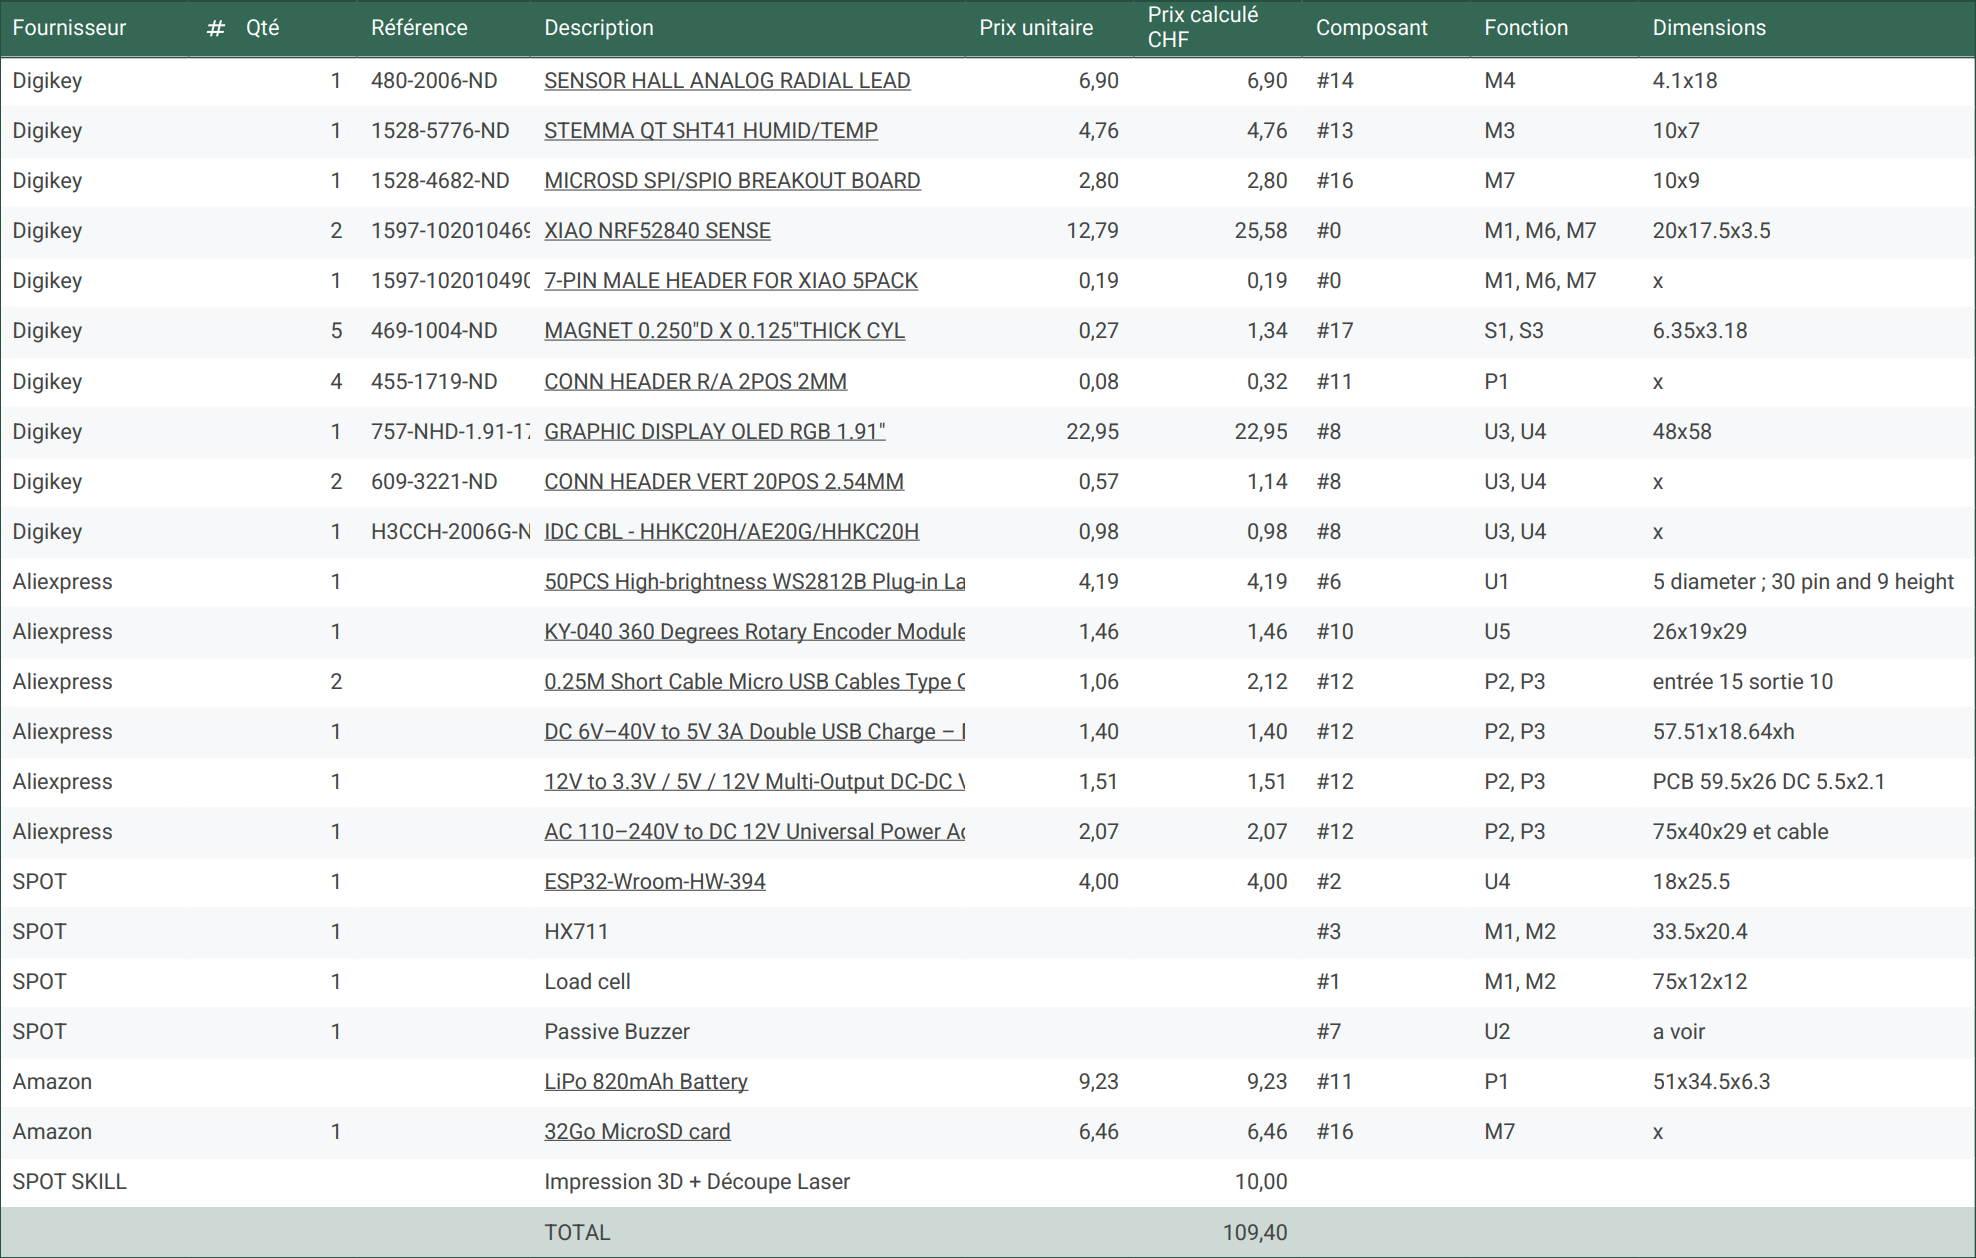
\includegraphics[
        width=0.9\paperwidth
    ]{Photos/prix.png}
    \caption{Table of components with detailed pricing.}
    \label{fig:pricing_components}
\end{figure}




% À compléter.

\subsection{How did you use AI?}

Artificial intelligence tools were used as a support tool throughout the project, mainly to improve efficiency, clarity, and structure, without replacing technical or creative decision-making. AI was primarily employed during the documentation, communication, and presentation phases of the project. It was used to help reformulate and clarify technical explanations, improve the quality of written english, and ensure coherence and structure in sections such as the executive summary, risk assessment descriptions, and project management reflections.\vspace{0.1cm}

AI was also used to support ideation and reasoning, for example by helping to explore alternative design solutions. In these cases, AI served as a brainstorming assistant, while all final decisions, validations, and implementations were carried out by the team. It also served as a coding assistant.\vspace{0.1cm}

Importantly, AI was not used to generate technical designs, simulations, or analytical results. All hardware design, system modeling, and experimental validation were performed manually by the team. The use of AI remained limited to assistance in writing, structuring, and refining content, ensuring that the technical work and intellectual contributions of the project are entirely original and fully owned by the team.\vspace{0.1cm}

This approach allowed us to save time on non-core tasks while maintaining full control over the engineering and design aspects of the project.

% À compléter si tu veux décrire l'utilisation de ChatGPT.
\newpage
\subsection{Technical drawings}
\textbf{Coaster :}\\
The CAD was made on CATIA then used in STL format to be used on PrusaSlicer to then 3D print the coaster.
\begin{figure}[H]
    \centering
    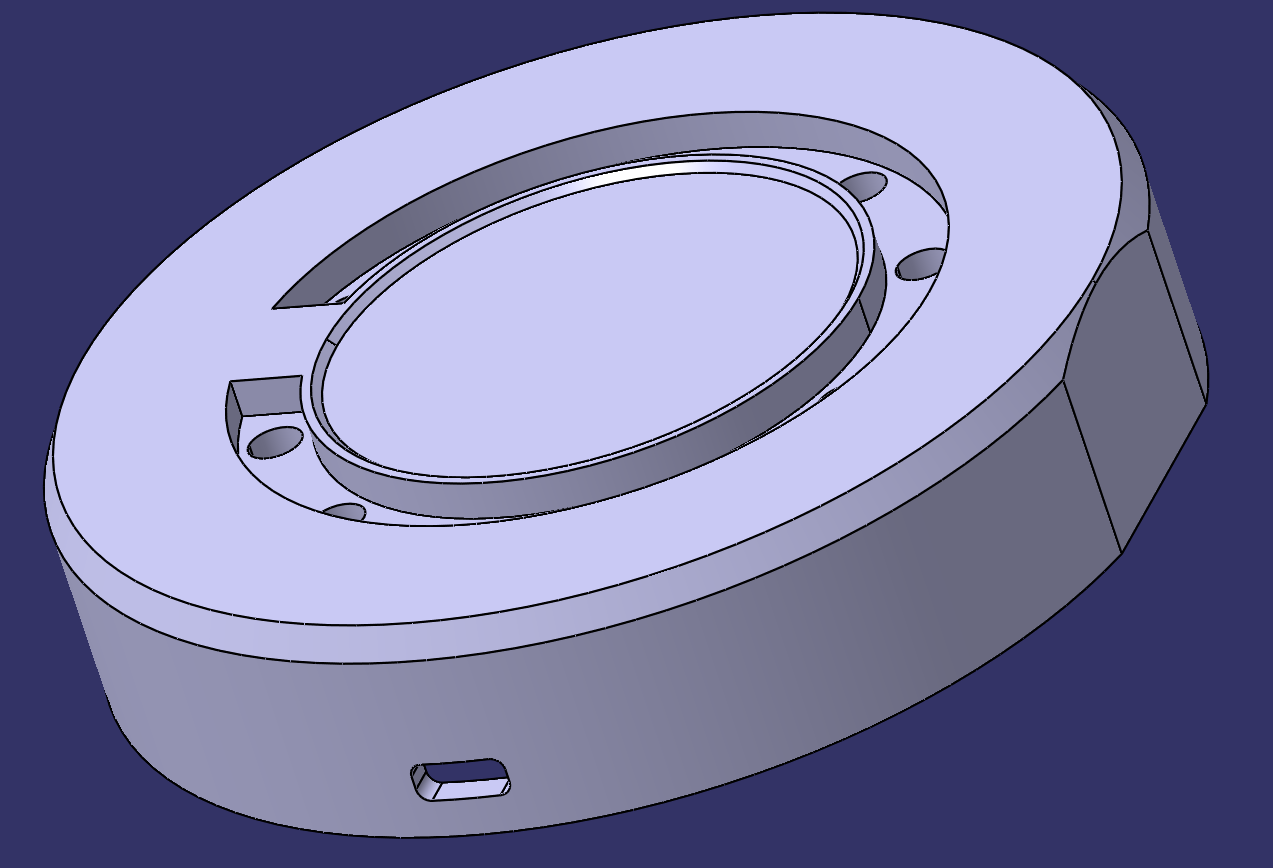
\includegraphics[width=0.85\textwidth]{Photos/vue_dessus.png}
    \caption{Top view of the coaster (CATIA Screenshot).}
    \label{fig:coaster_dessus}
\end{figure}

\begin{figure}[H]
    \centering
    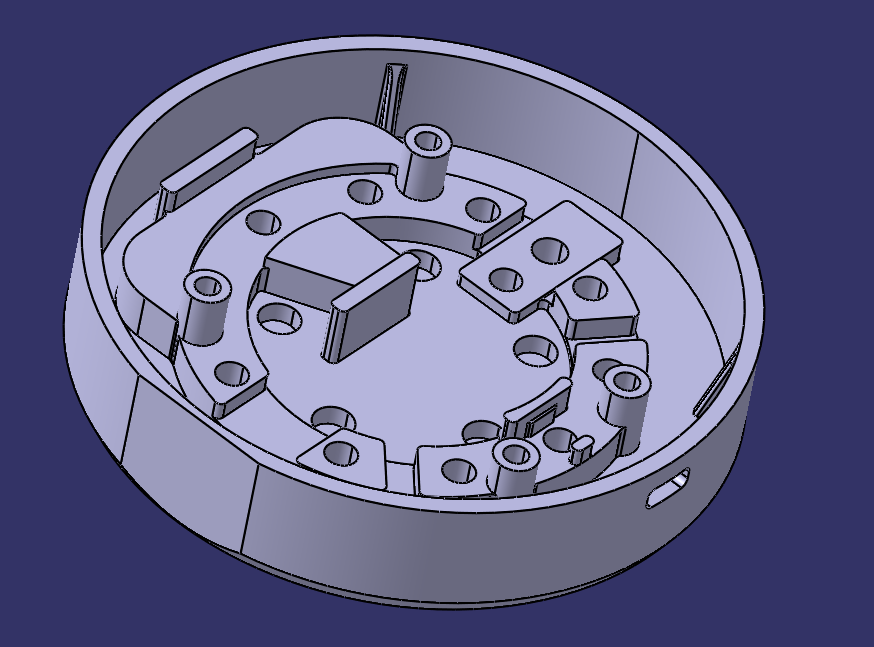
\includegraphics[width=0.85\textwidth]{Photos/vue_dessous.png}
    \caption{Underneath view of the coaster (CATIA Screenshot).}
    \label{fig:coaster_dessous}
\end{figure}
\newpage
\textbf{Base :}\\

\begin{figure}[H]
    \centering
    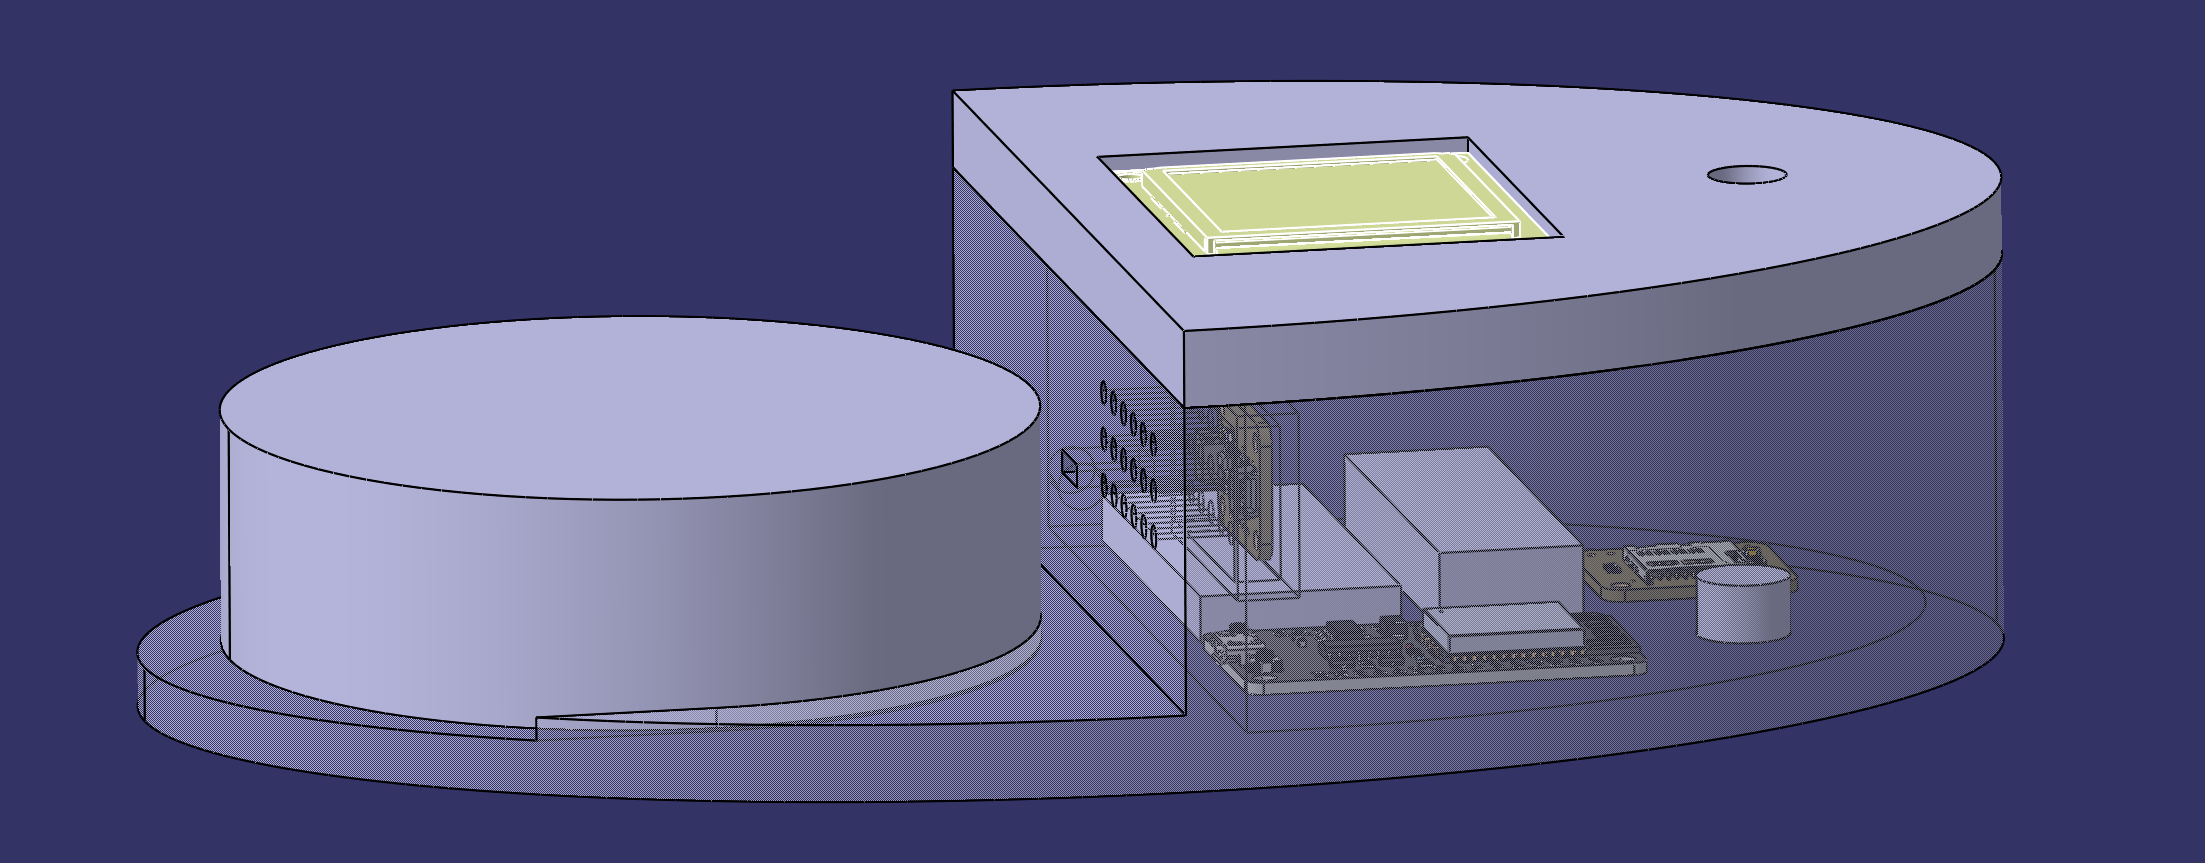
\includegraphics[width=1\textwidth]{Photos/vue ensemble.png}
    \caption{Base + Coaster CAD model (CATIA Screenshot).}
    \label{fig:base+coaster}
\end{figure}

\begin{figure}[H]
    \centering
    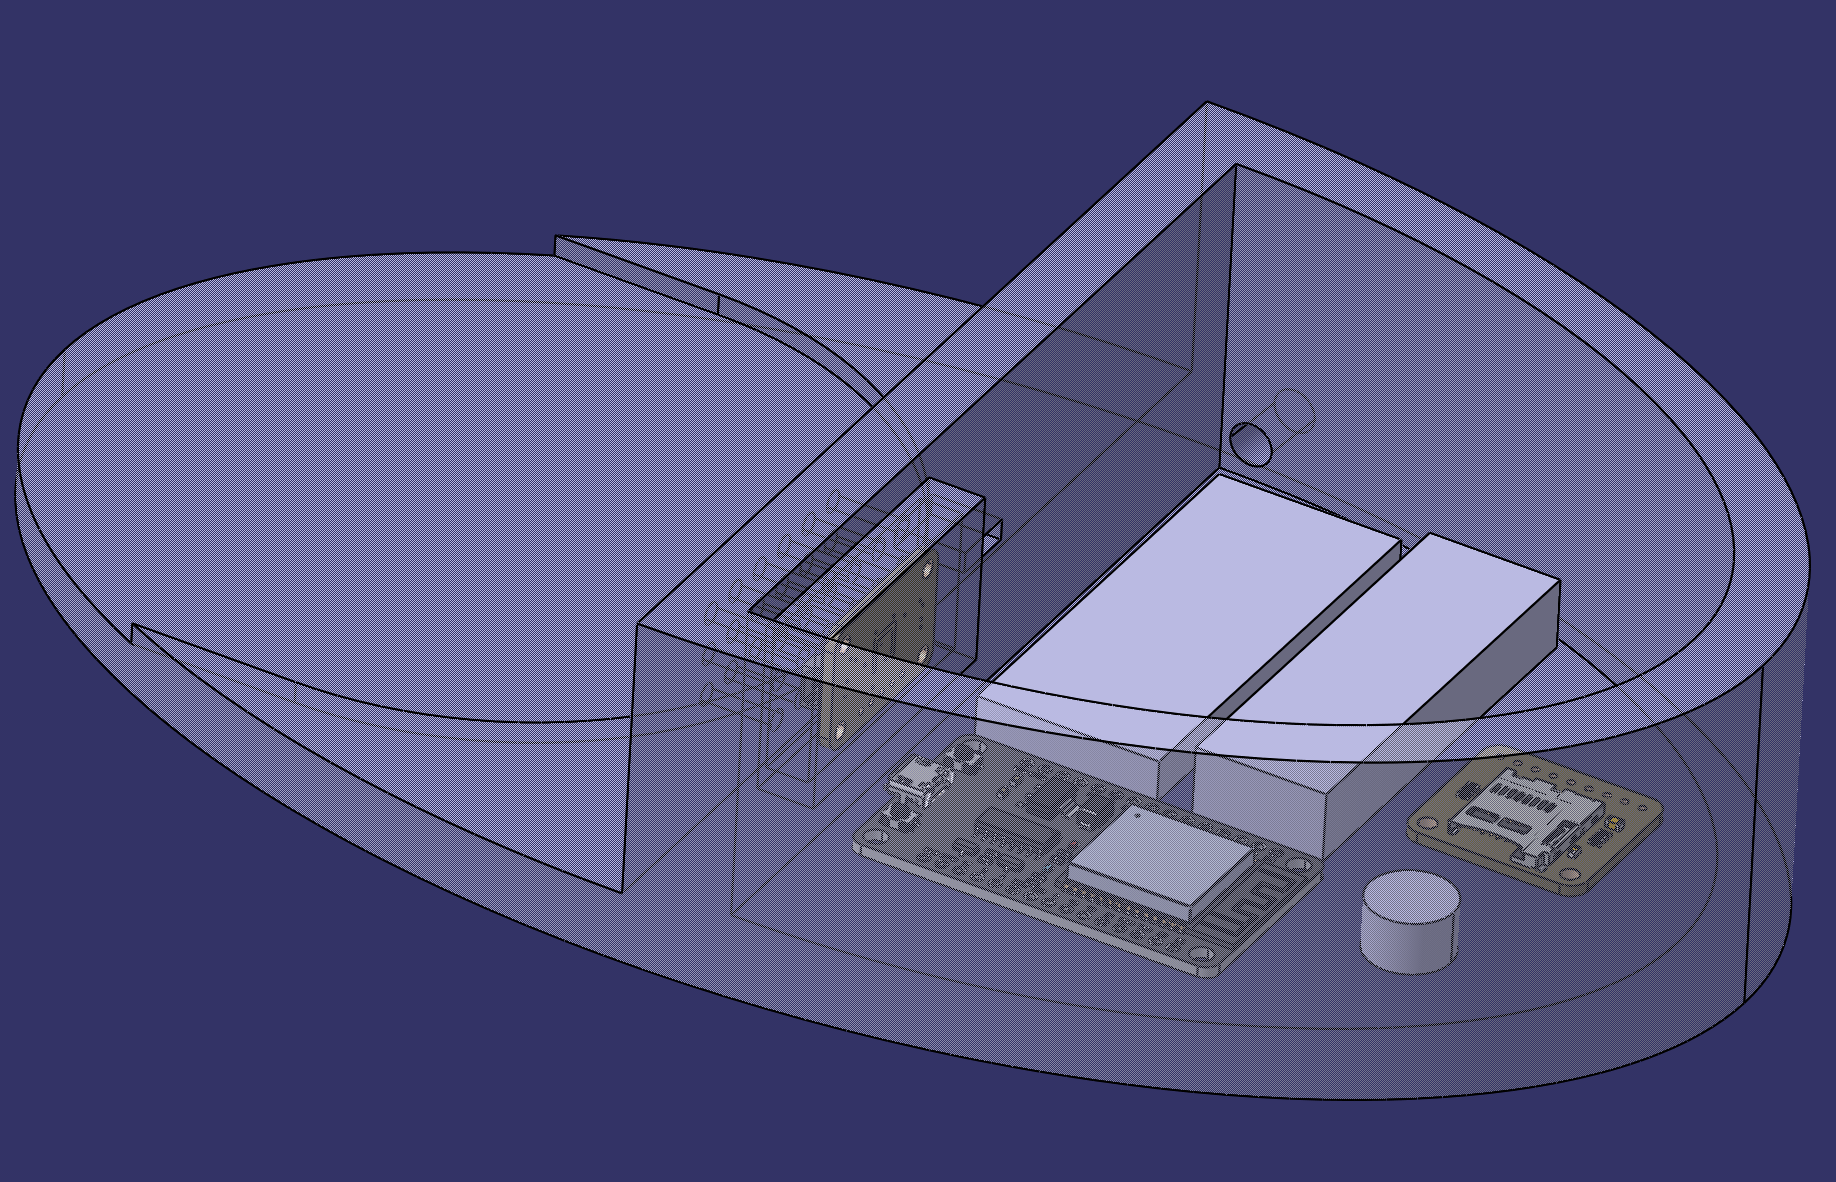
\includegraphics[width=1\textwidth]{Photos/vue interieure.png}
    \caption{Internal component architecture of the Base (CATIA Screenshot).}
    \label{fig:base}
\end{figure}

\begin{figure}[H]
    \centering
    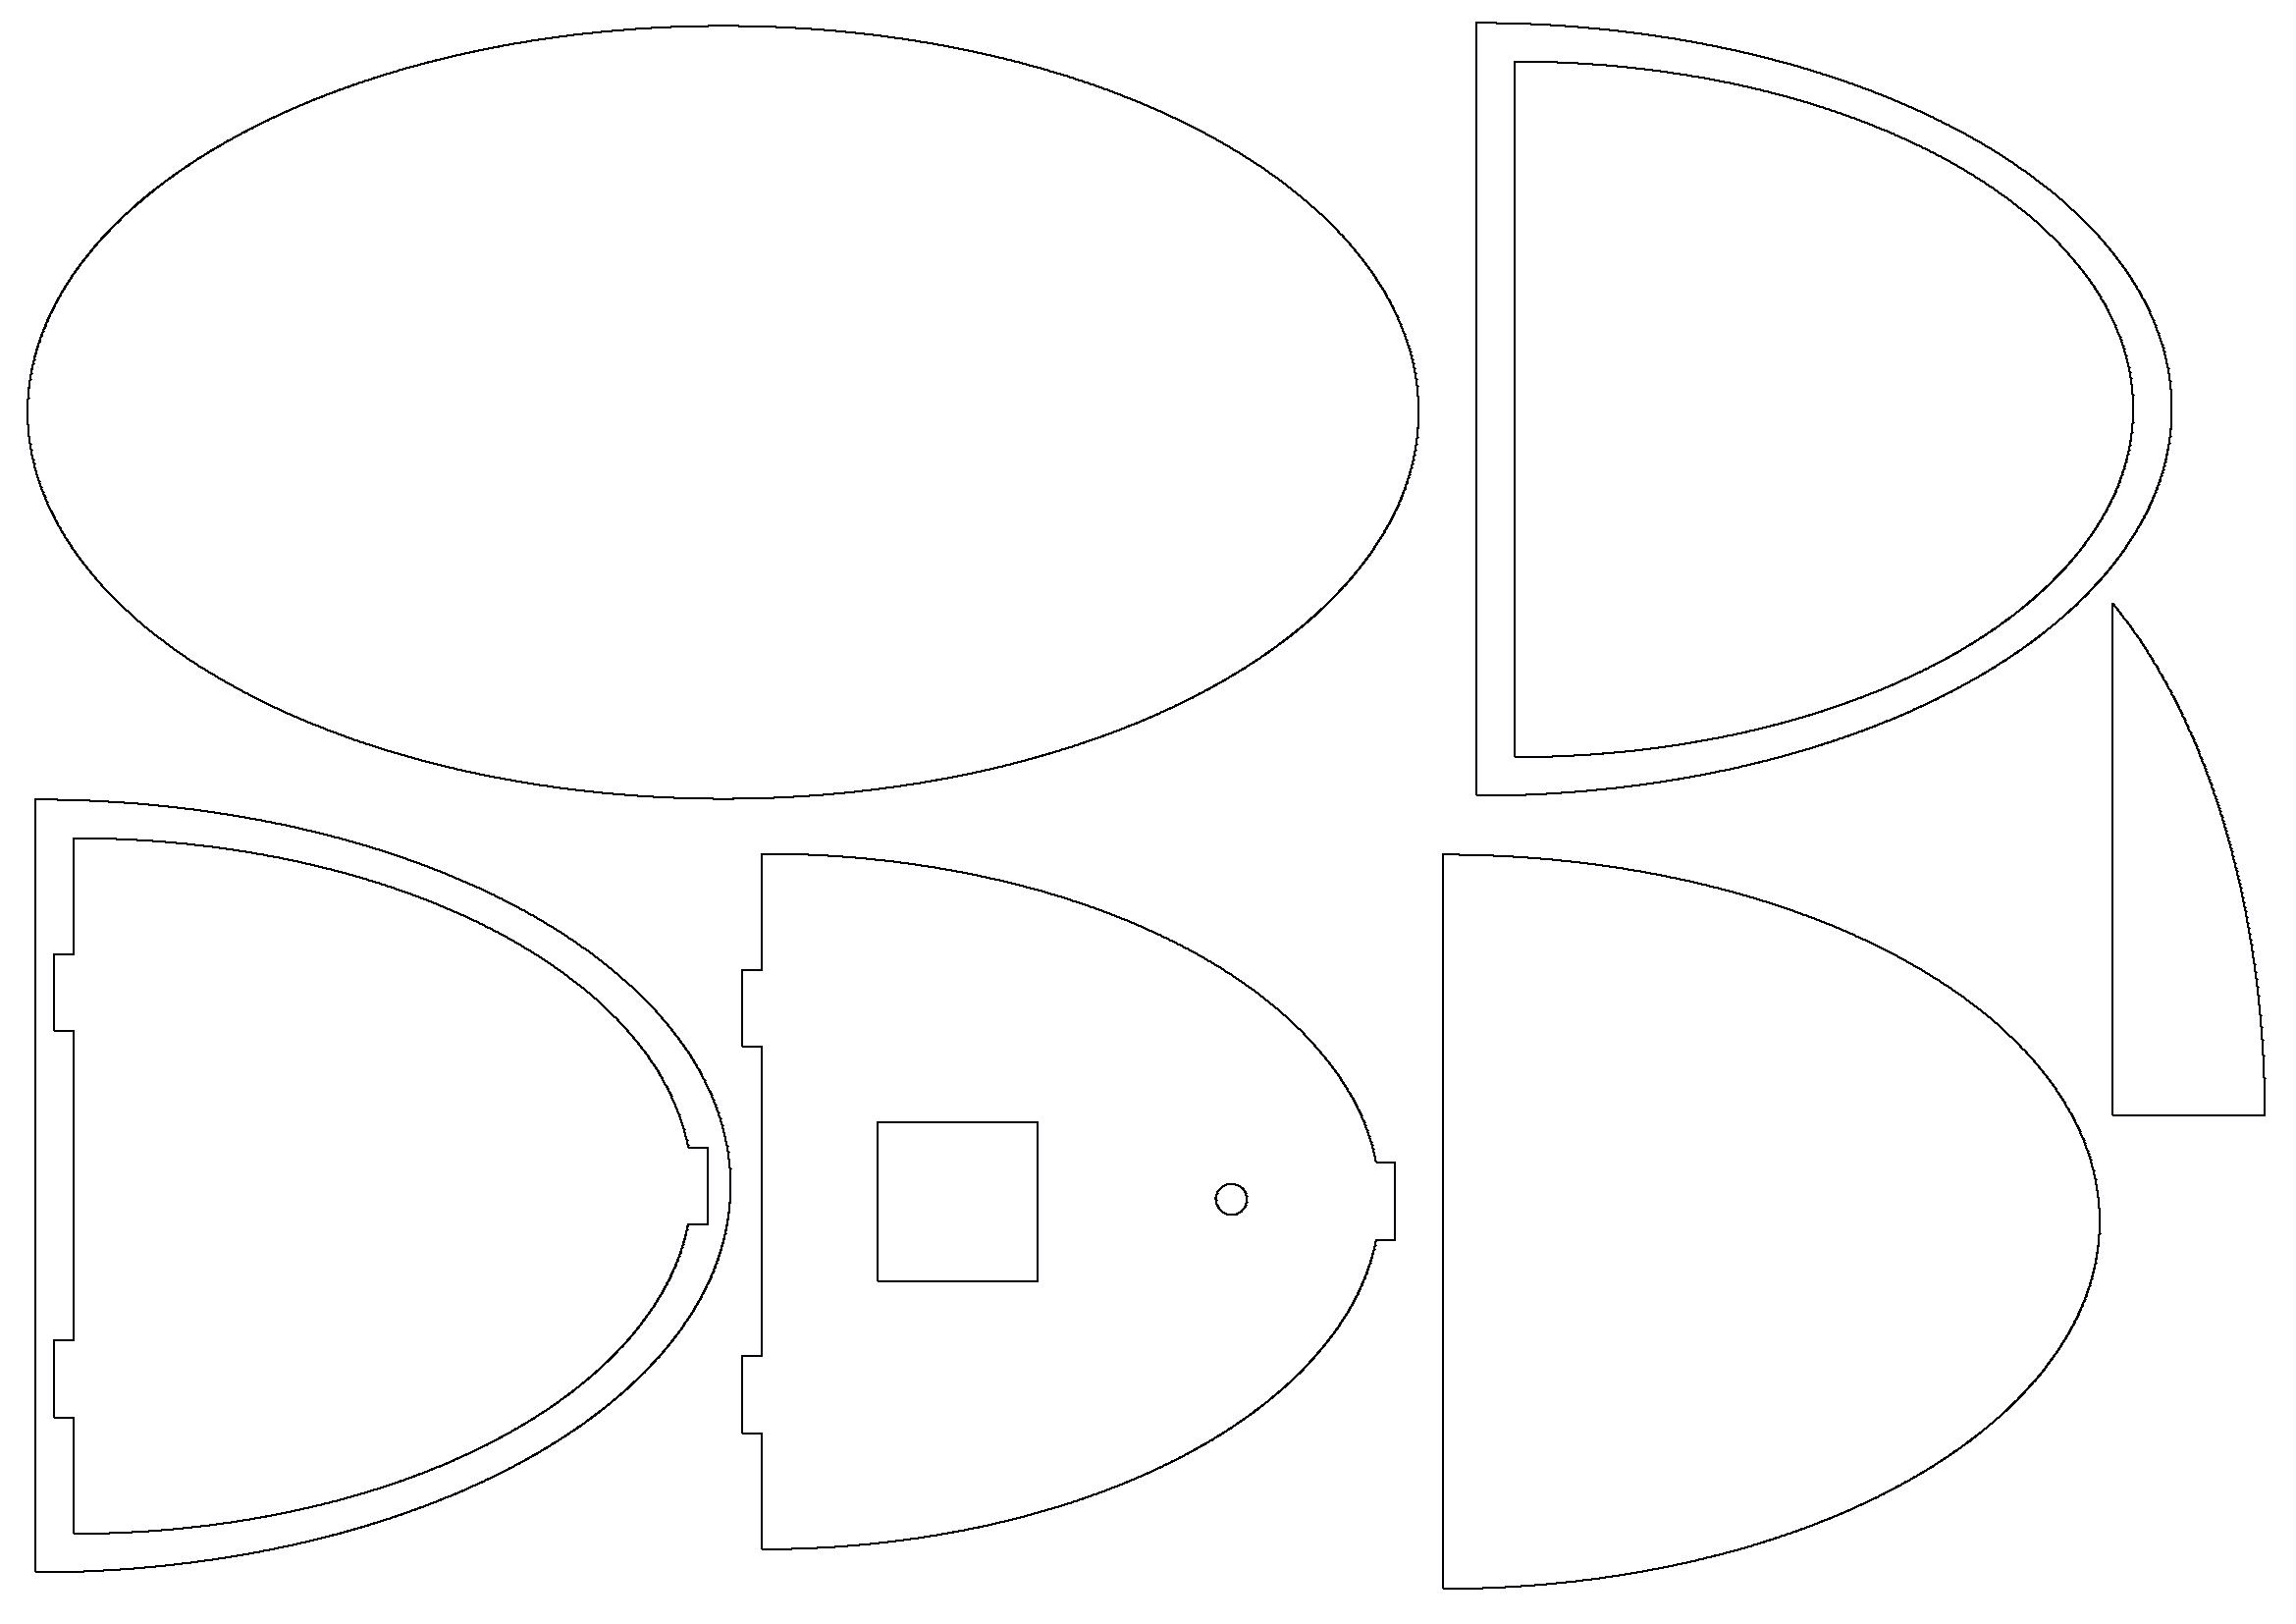
\includegraphics[width=1\textwidth]{Photos/pieces.jpg}
    \caption{DXF file showing all laser-cut parts for base assembly.}
    \label{fig:dxf_base}
\end{figure}

% À compléter avec les dessins techniques finaux.

\subsection{Circuit diagrams}

\begin{figure}[H]
    \centering
    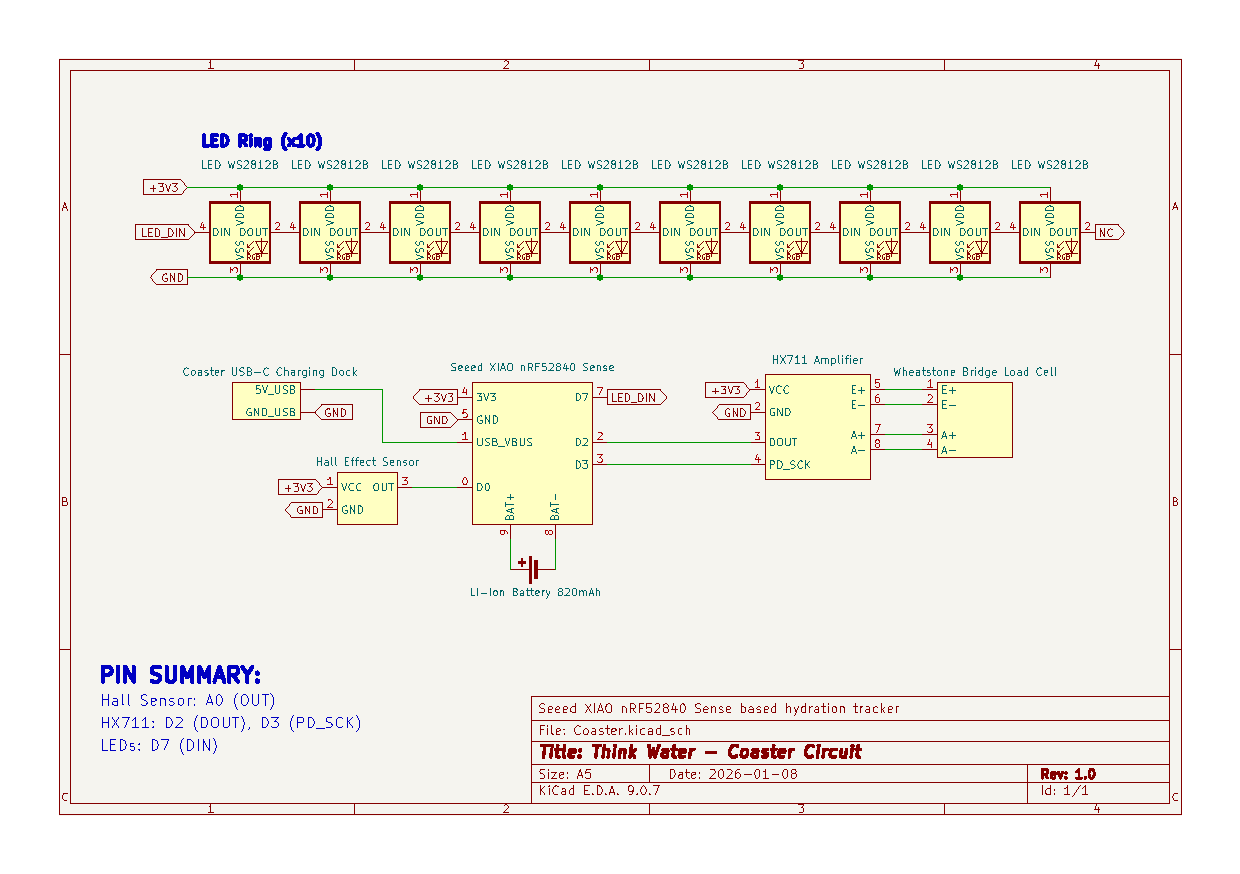
\includegraphics[width=1\textwidth]{Schematics/Coaster.pdf}
    \caption{Coaster circuit schematic showing the Seeed XIAO nRF52840 Sense microcontroller with HX711 load cell amplifier, Hall effect sensor for glass detection, and WS2812B NeoPixel LED ring for visual feedback.}
    \label{fig:coaster-circuit}
\end{figure}

\begin{figure}[H]
    \centering
    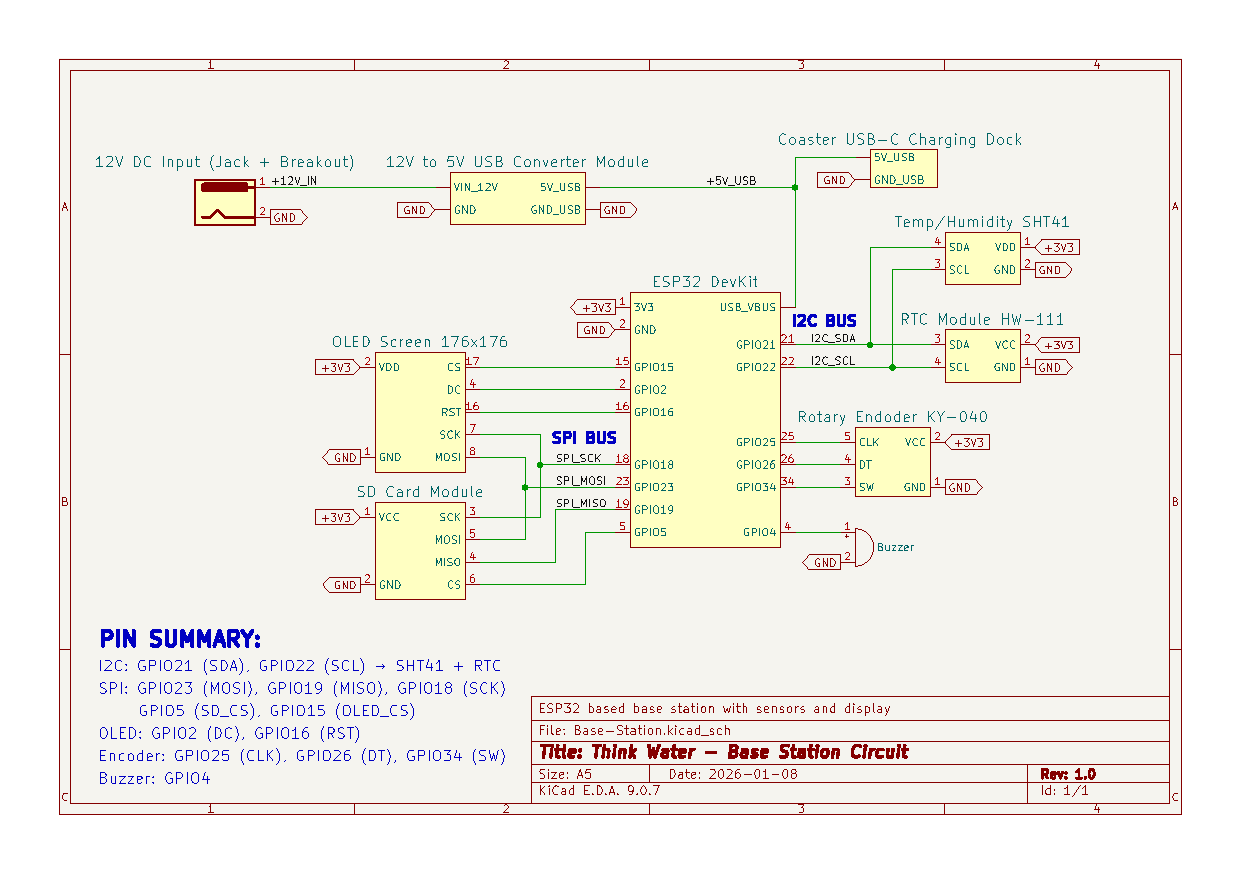
\includegraphics[width=1\textwidth]{Schematics/Base-Station.pdf}
    \caption{Base station circuit schematic showing the ESP32 microcontroller with I2C peripherals (SHT41 temperature/humidity sensor and HW-111 RTC), SPI peripherals (SD card module and SSD1333 OLED display), rotary encoder for user input, and active buzzer for audio alerts.}
    \label{fig:base-circuit}
\end{figure}

\subsection{Logo}

\begin{figure}[H]
    \centering
    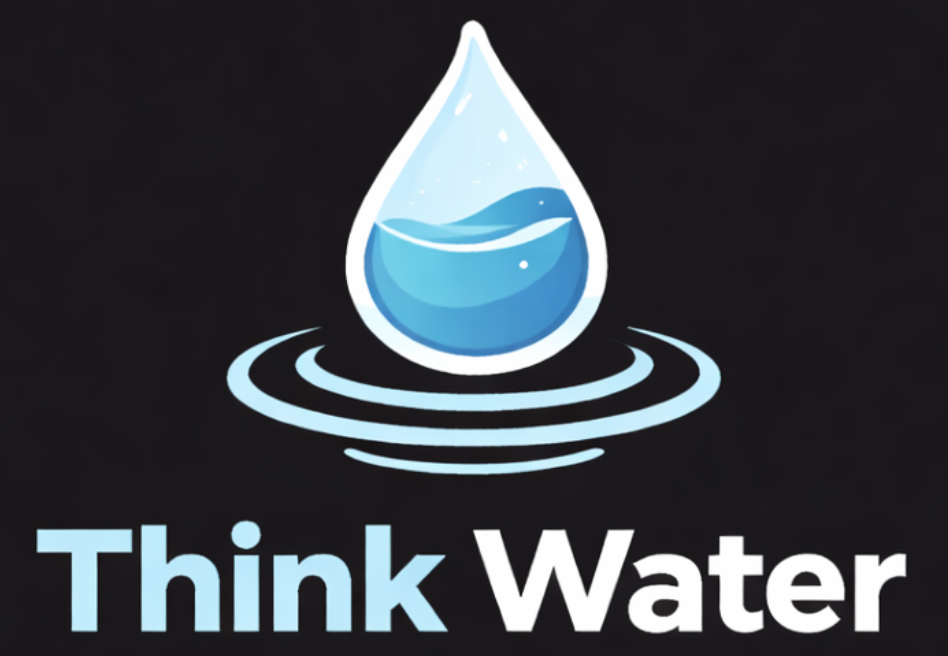
\includegraphics[width=0.6\textwidth]{logos/logo_avec _fond.png}
    \caption{Logo of the "Think Water" company}
    \label{fig:logogo}
\end{figure}
% Toute info supplémentaire (algos, simulations, etc.)


%\pagebreak


\newpage

\printbibliography[heading=bibintoc]
%\printbibliography[heading=bibintoc] 


\phantomsection
\label{appendix:FirstClaim}
\includepdf[
  pages=-,
  pagecommand={
    \thispagestyle{empty}
    \begin{tikzpicture}[remember picture,overlay]
      \node[anchor=north,yshift=-1cm] at (current page.north)
        {\LARGE\bfseries IP first claim};
    \end{tikzpicture}
  }
]{IP First claims.pdf}

\phantomsection
\label{appendix:interview}
\includepdf[
  pages=-,
  pagecommand={
    \thispagestyle{empty}
    \begin{tikzpicture}[remember picture,overlay]
      \node[anchor=north,yshift=-1cm] at (current page.north)
        {\LARGE\bfseries Interview with doctors};
    \end{tikzpicture}
  }
]{Interview.pdf}

\end{document}
